% !TeX program = pdflatex
\documentclass[12pt,a4paper]{article}

\usepackage[utf8]{inputenc}
\usepackage[T1]{fontenc}
\usepackage[polish]{babel}
\usepackage{graphicx}
\usepackage{amsmath, amssymb}
\usepackage{float}
\usepackage{geometry}
\usepackage{booktabs}
\usepackage{caption}
\usepackage{subcaption}
\usepackage{pgfplots}
\usepackage{hyperref}
\usepackage{icomma}
\usepackage{tikz}
\usetikzlibrary{shapes, arrows.meta, positioning, calc}

\geometry{margin=2.5cm}
\setlength{\parindent}{1.2cm}
\setlength{\parskip}{0.5em}
\linespread{1.2}
\pgfplotsset{compat=1.18}

\hypersetup{
	colorlinks=true,
	linkcolor=black,
	filecolor=black,
	urlcolor=blue,
	pdftitle={Sprawozdanie SA - Cw 2},
	pdfpagemode=FullScreen,
}

\begin{document}
		\begin{titlepage}
		\centering
		\Huge \textbf{Sprawozdanie z ćwiczeń laboratoryjnych}\\[0.5cm]
		\Large z przedmiotu: \textit{Sterowanie Analogowe}\\[2cm]
		
		\begin{tabular}{|p{6cm}|p{10cm}|}
			\hline
			\textbf{Numer ćwiczenia:} & 2 \\ \hline
			\textbf{Tytuł ćwiczenia:} & Badanie jakości i dokładności sterowania \\ \hline
			\textbf{Imię, nazwisko i numer albumu:} &
			\begin{tabular}[t]{@{}l@{}}
				Mateusz Kuczerowski 197900\\
				Kewin Kisiel 197866\\
			\end{tabular} \\ \hline
			\textbf{Data pomiarów:} & 16.10.2025 \\ \hline
			\textbf{Data oddania:} & 25.10.2025 \\ \hline
			\textbf{Ocena:} & \\ \hline
		\end{tabular}\\[2cm]
		
		\vfill
		\textbf{Prowadzący:} dr inż. Piotr Fiertek\\[0.2cm]
		\textbf{Grupa laboratoryjna:} 1A\\[1cm]
	\end{titlepage}
	
	\section{Cel ćwiczenia}
	W ramach zajęć analizowano odpowiedzi skokowe oraz charakterystyki częstotliwościowe (Bodego) dla różnych wartości wzmocnienia. Pozwoliło to na ocenę, jak zmiana $k_c$ wpływa na parametry odpowiedzi, takie jak przeregulowanie, czas ustalania, pasmo przenoszenia oraz dokładność sterowania (uchyb ustalony).
	
	\section{Przebieg ćwiczenia}
	Podczas ćwiczenia przeprowadzono badanie trzech różnych układów zamkniętych (Układ A, B, D), wskazanych przez prowadzącego. Układy te były sterowane za pomocą sterownika proporcjonalnego (P).
	Dla każdego z badanych układów zarejestrowano łącznie 9 odpowiedzi skokowych – po trzy dla każdej z trzech różnych wartości wzmocnienia sterownika $k_c$. W trakcie zajęć wykorzystano stanowisko pomiarowe składające się z zestawu analogowych modeli procesów przemysłowych (ZAMPP), generatora funkcji oraz oscyloskopu dwukanałowego. Zarejestrowane na oscyloskopie przebiegi (dane pomiarowe) zostały następnie wykorzystane do porównania z wynikami symulacji teoretycznych. Opracowanie wyników wymagało również przygotowania wykresów Nyquista oraz linii pierwiastkowych dla badanych układów.
	
	\newpage
	\section{Pomiary i analiza wyników}
	Poniżej przedstawiono zdjęcia z przeprowadzonych pomiarów w trakcie laboratorium.
	
	\begin{figure}[H]
		\centering
		\begin{subfigure}[b]{0.46\textwidth}
			\centering
			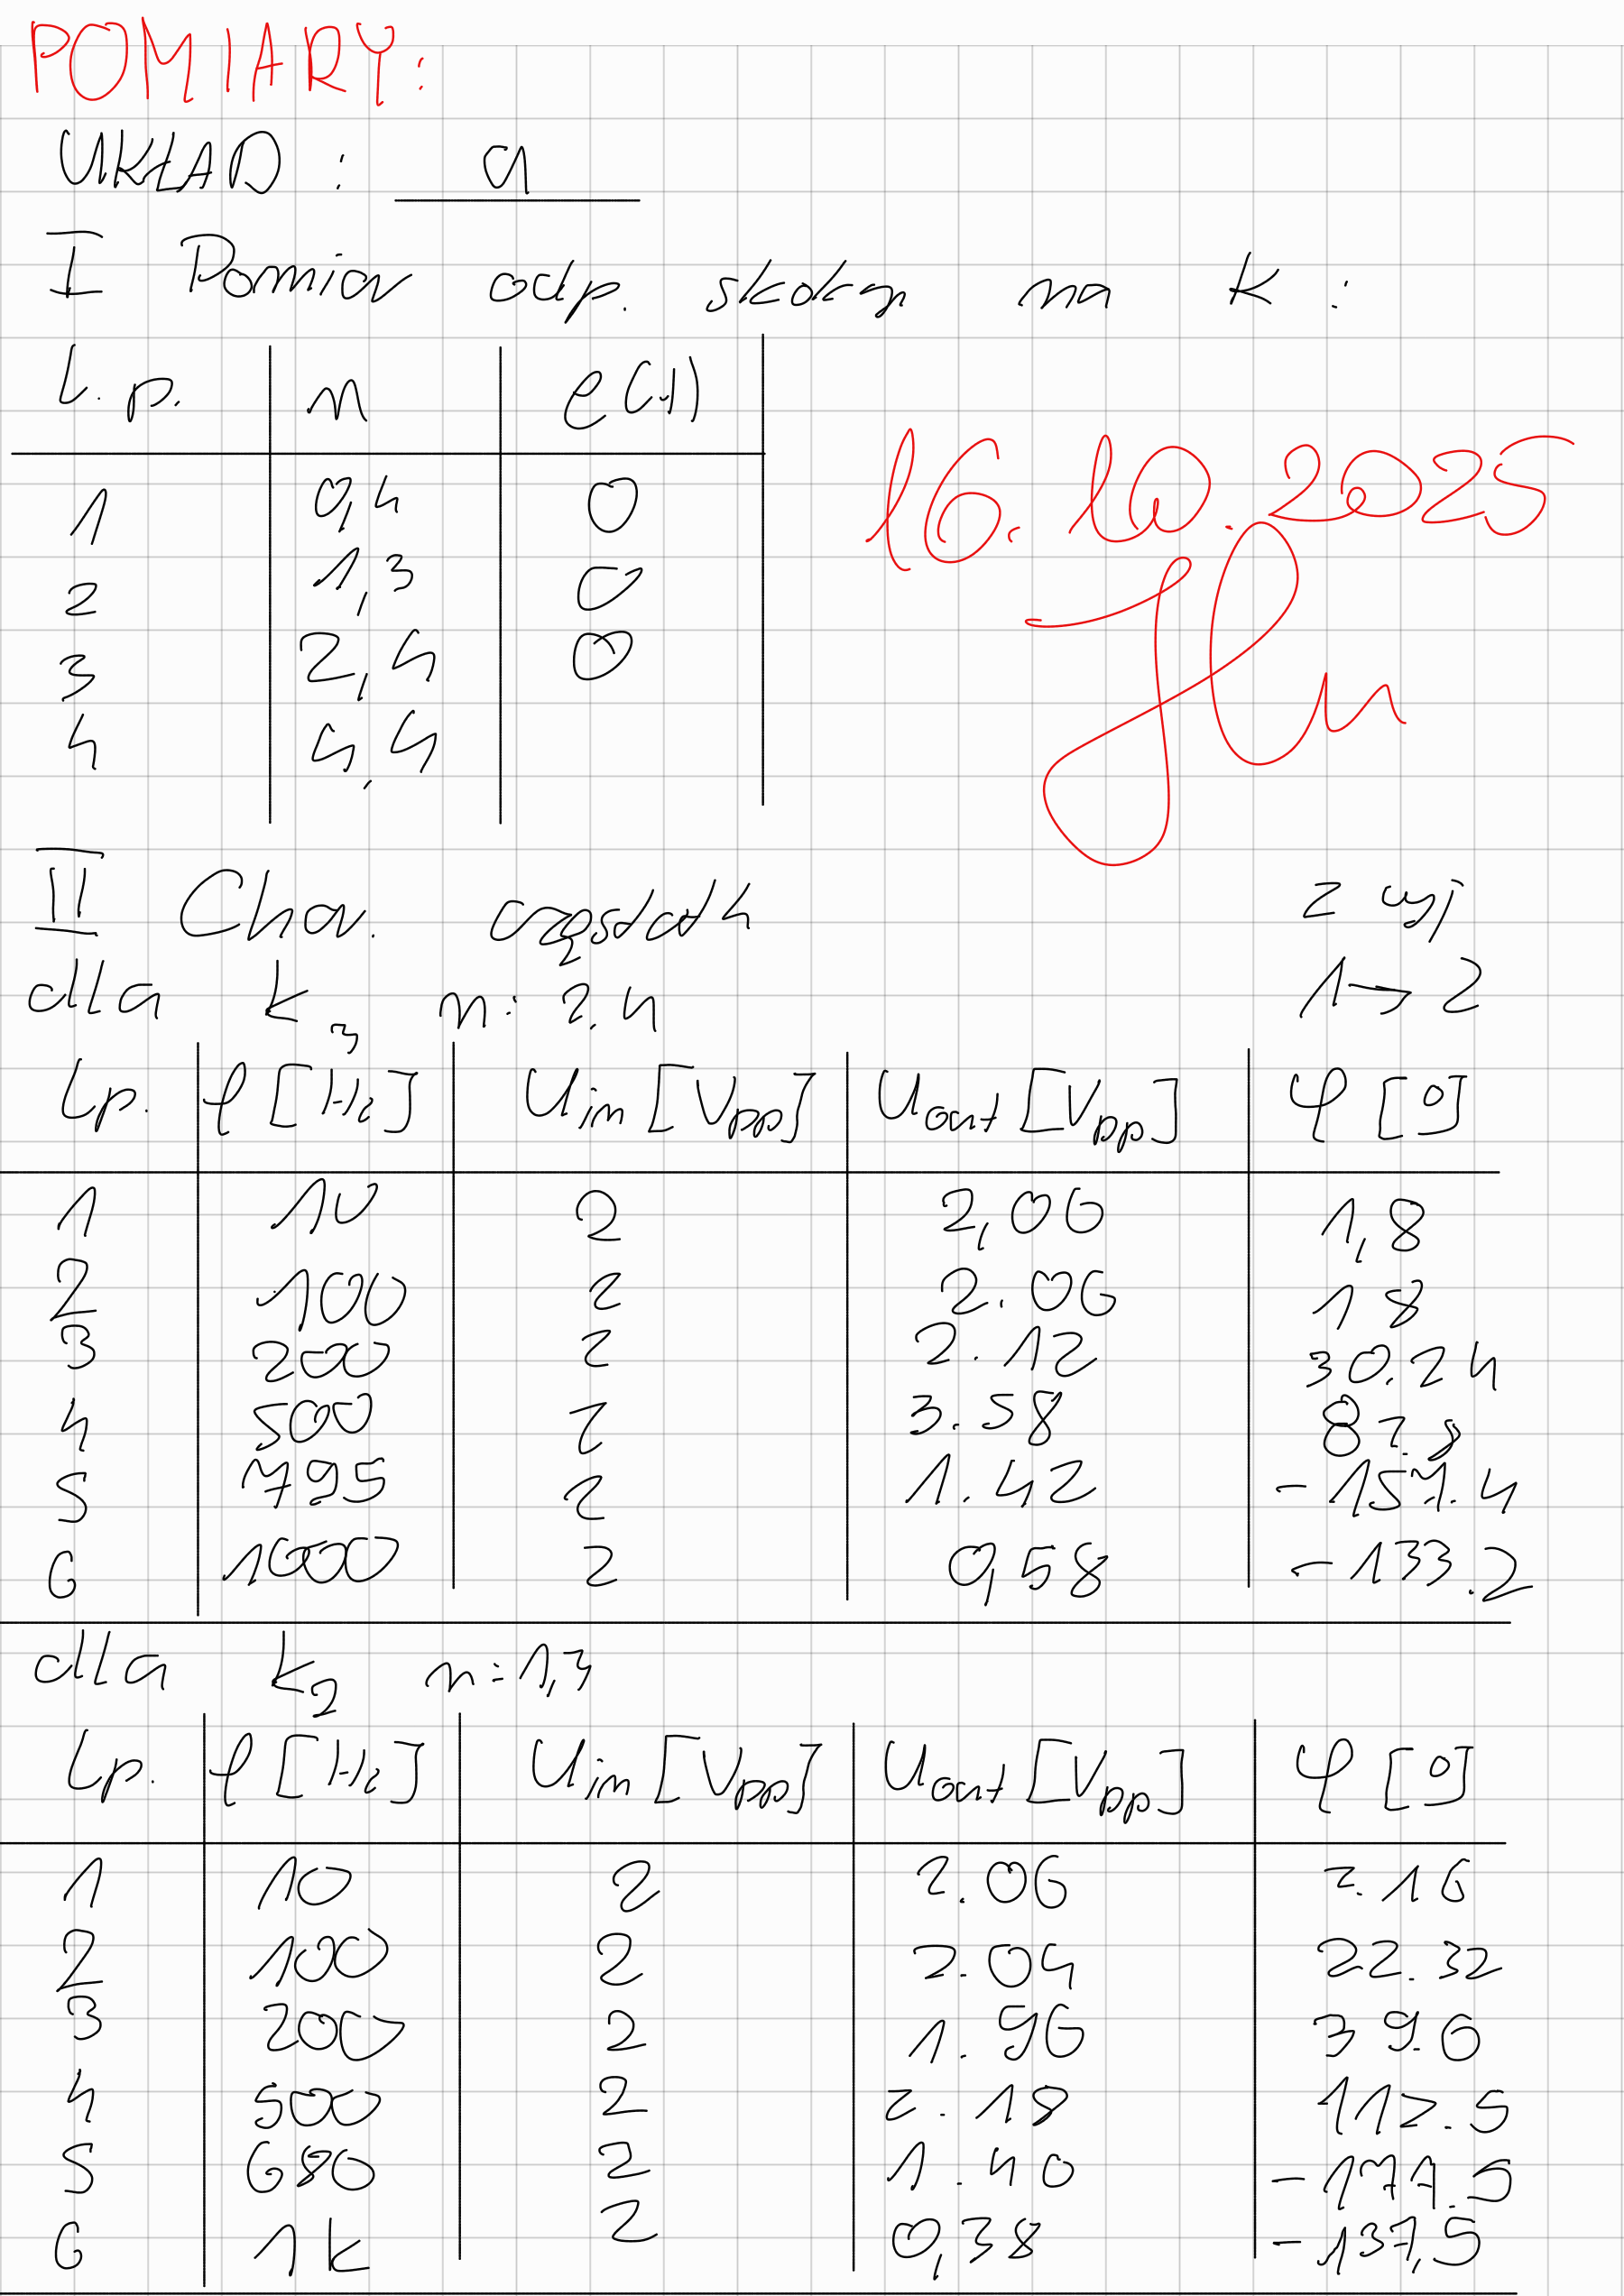
\includegraphics[width=\textwidth]{zdjecia/1.png}
			\caption{Zdjęcie pomiarów 1.}
			\label{fig:pomiar1}
		\end{subfigure}
		\hfill
		\begin{subfigure}[b]{0.46\textwidth}
			\centering
			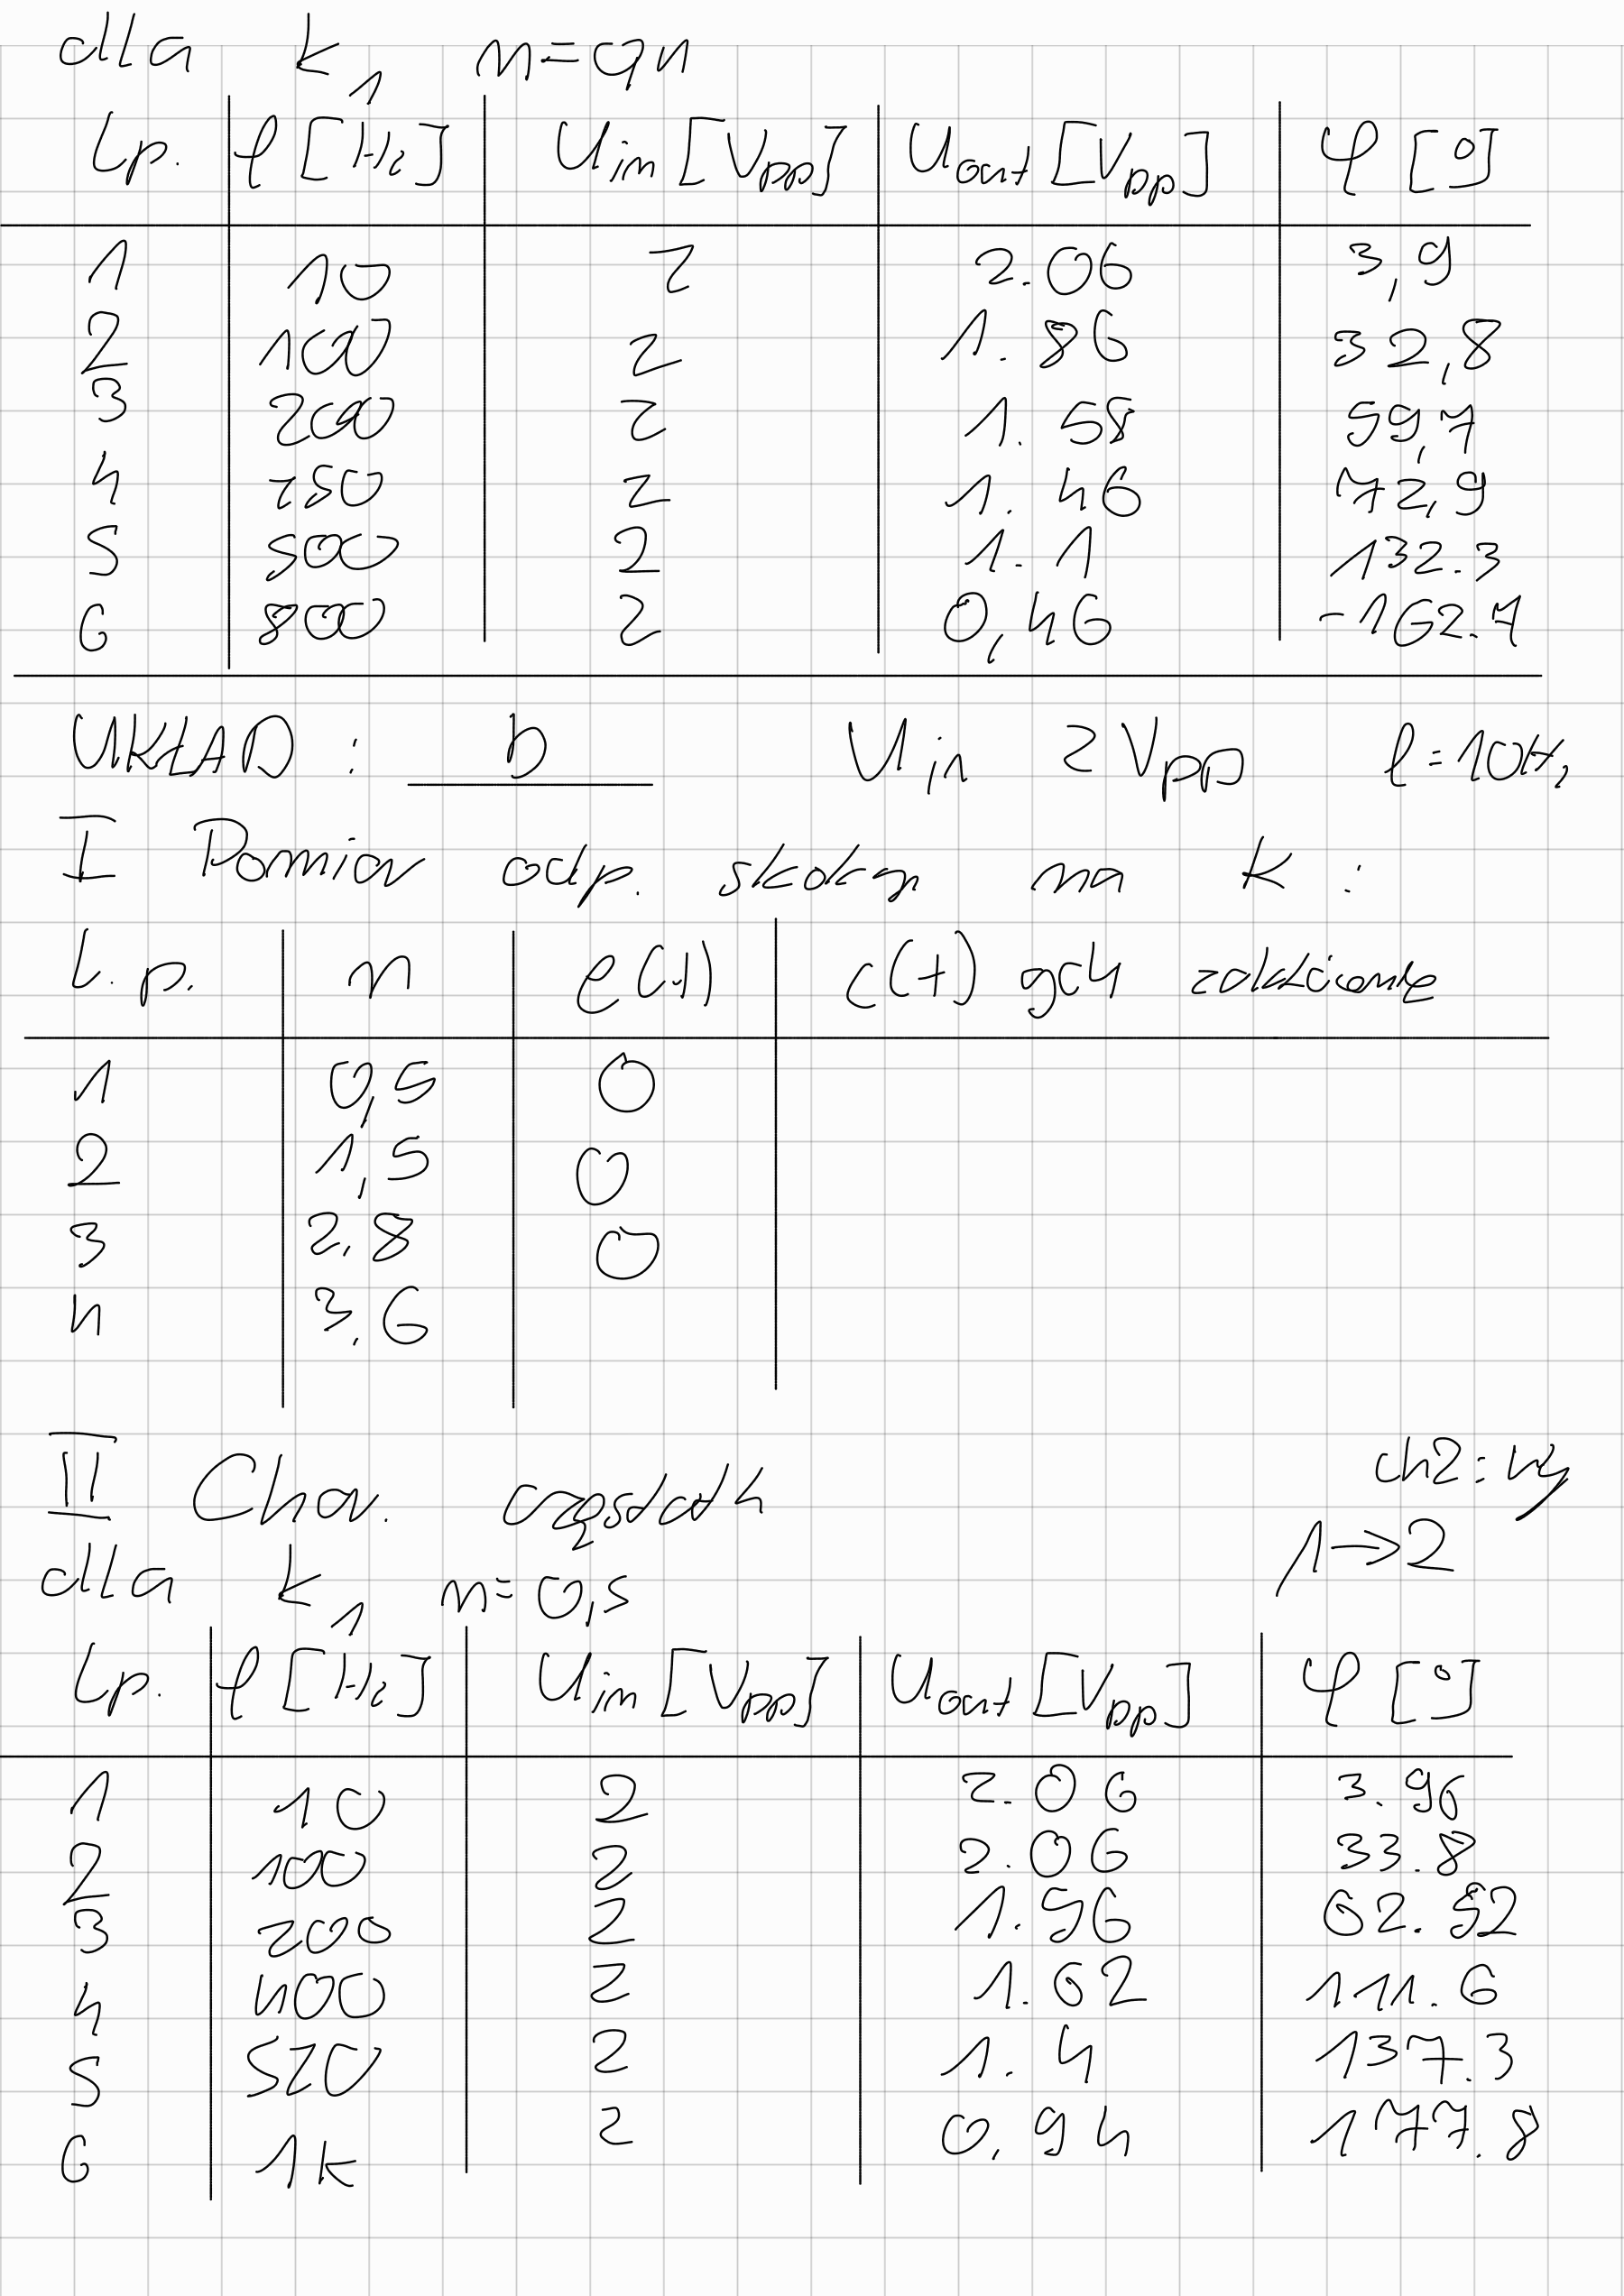
\includegraphics[width=\textwidth]{zdjecia/2.png}
			\caption{Zdjęcie pomiarów 2.}
			\label{fig:pomiar2}
		\end{subfigure}
		\begin{subfigure}[b]{0.46\textwidth}
			\centering
			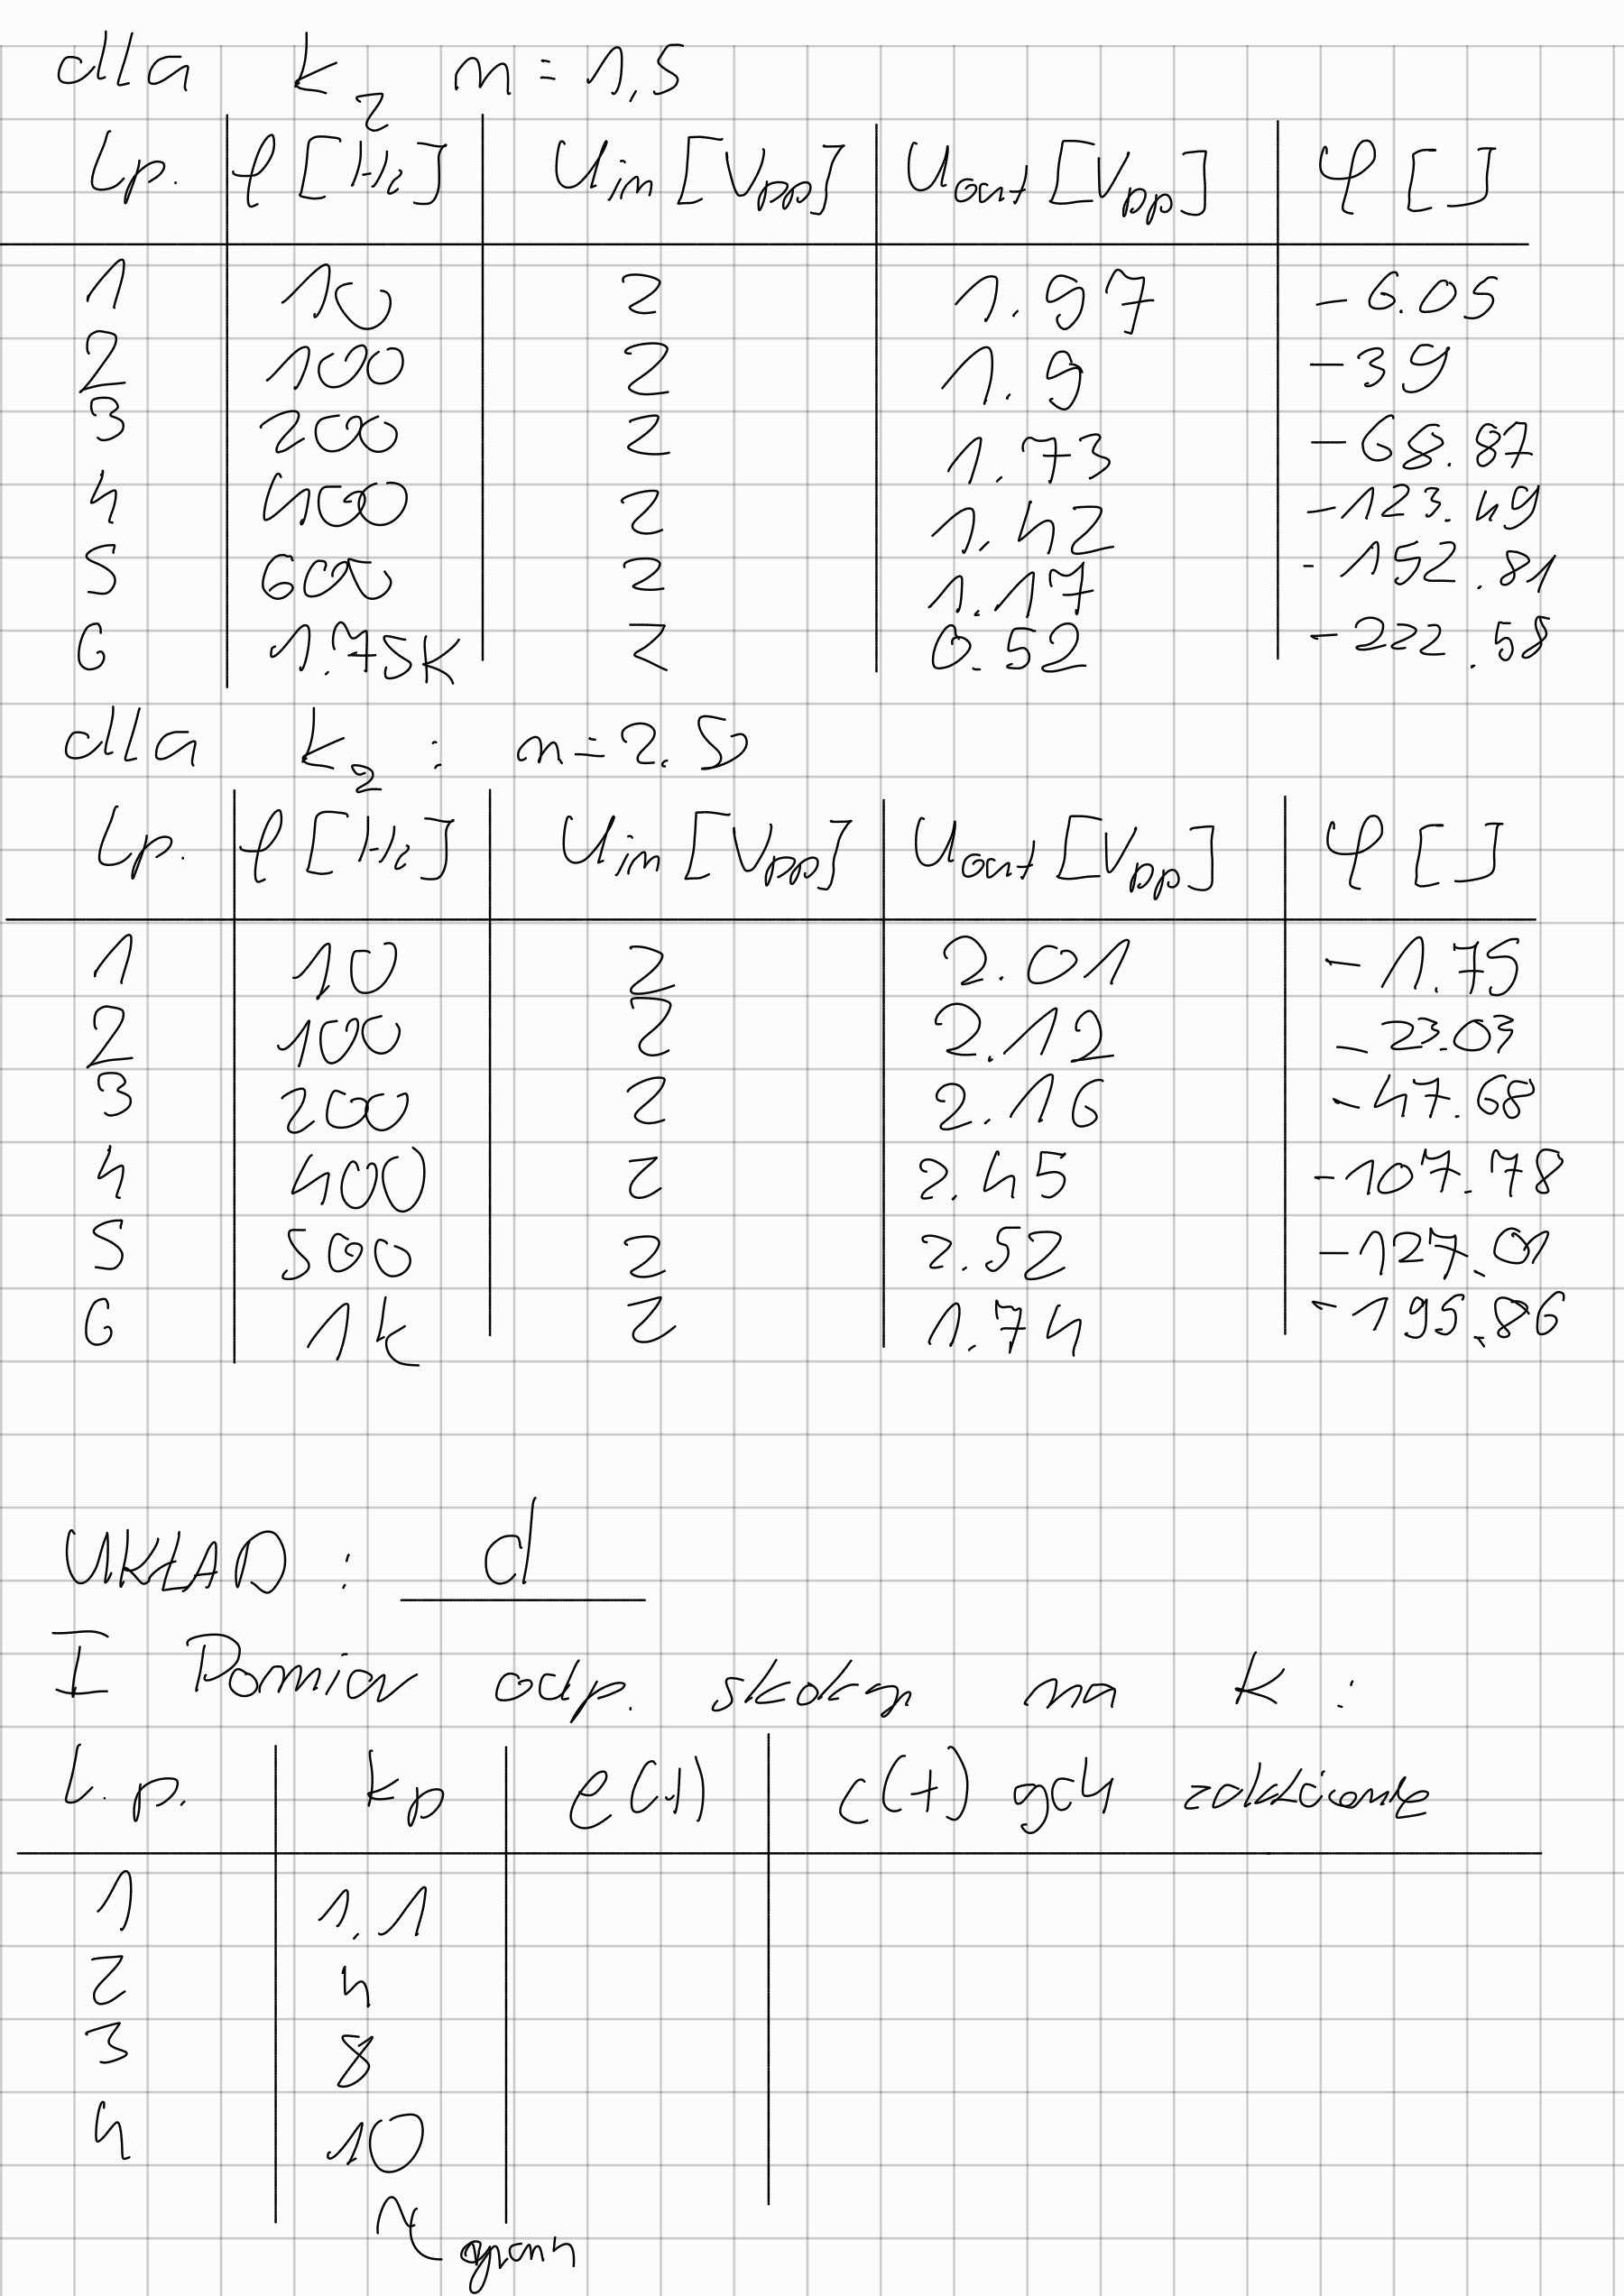
\includegraphics[width=\textwidth]{zdjecia/3.png}
			\caption{Zdjęcie pomiarów 3.}
			\label{fig:pomiar3}
		\end{subfigure}
		\hfill
		\begin{subfigure}[b]{0.46\textwidth}
			\centering
			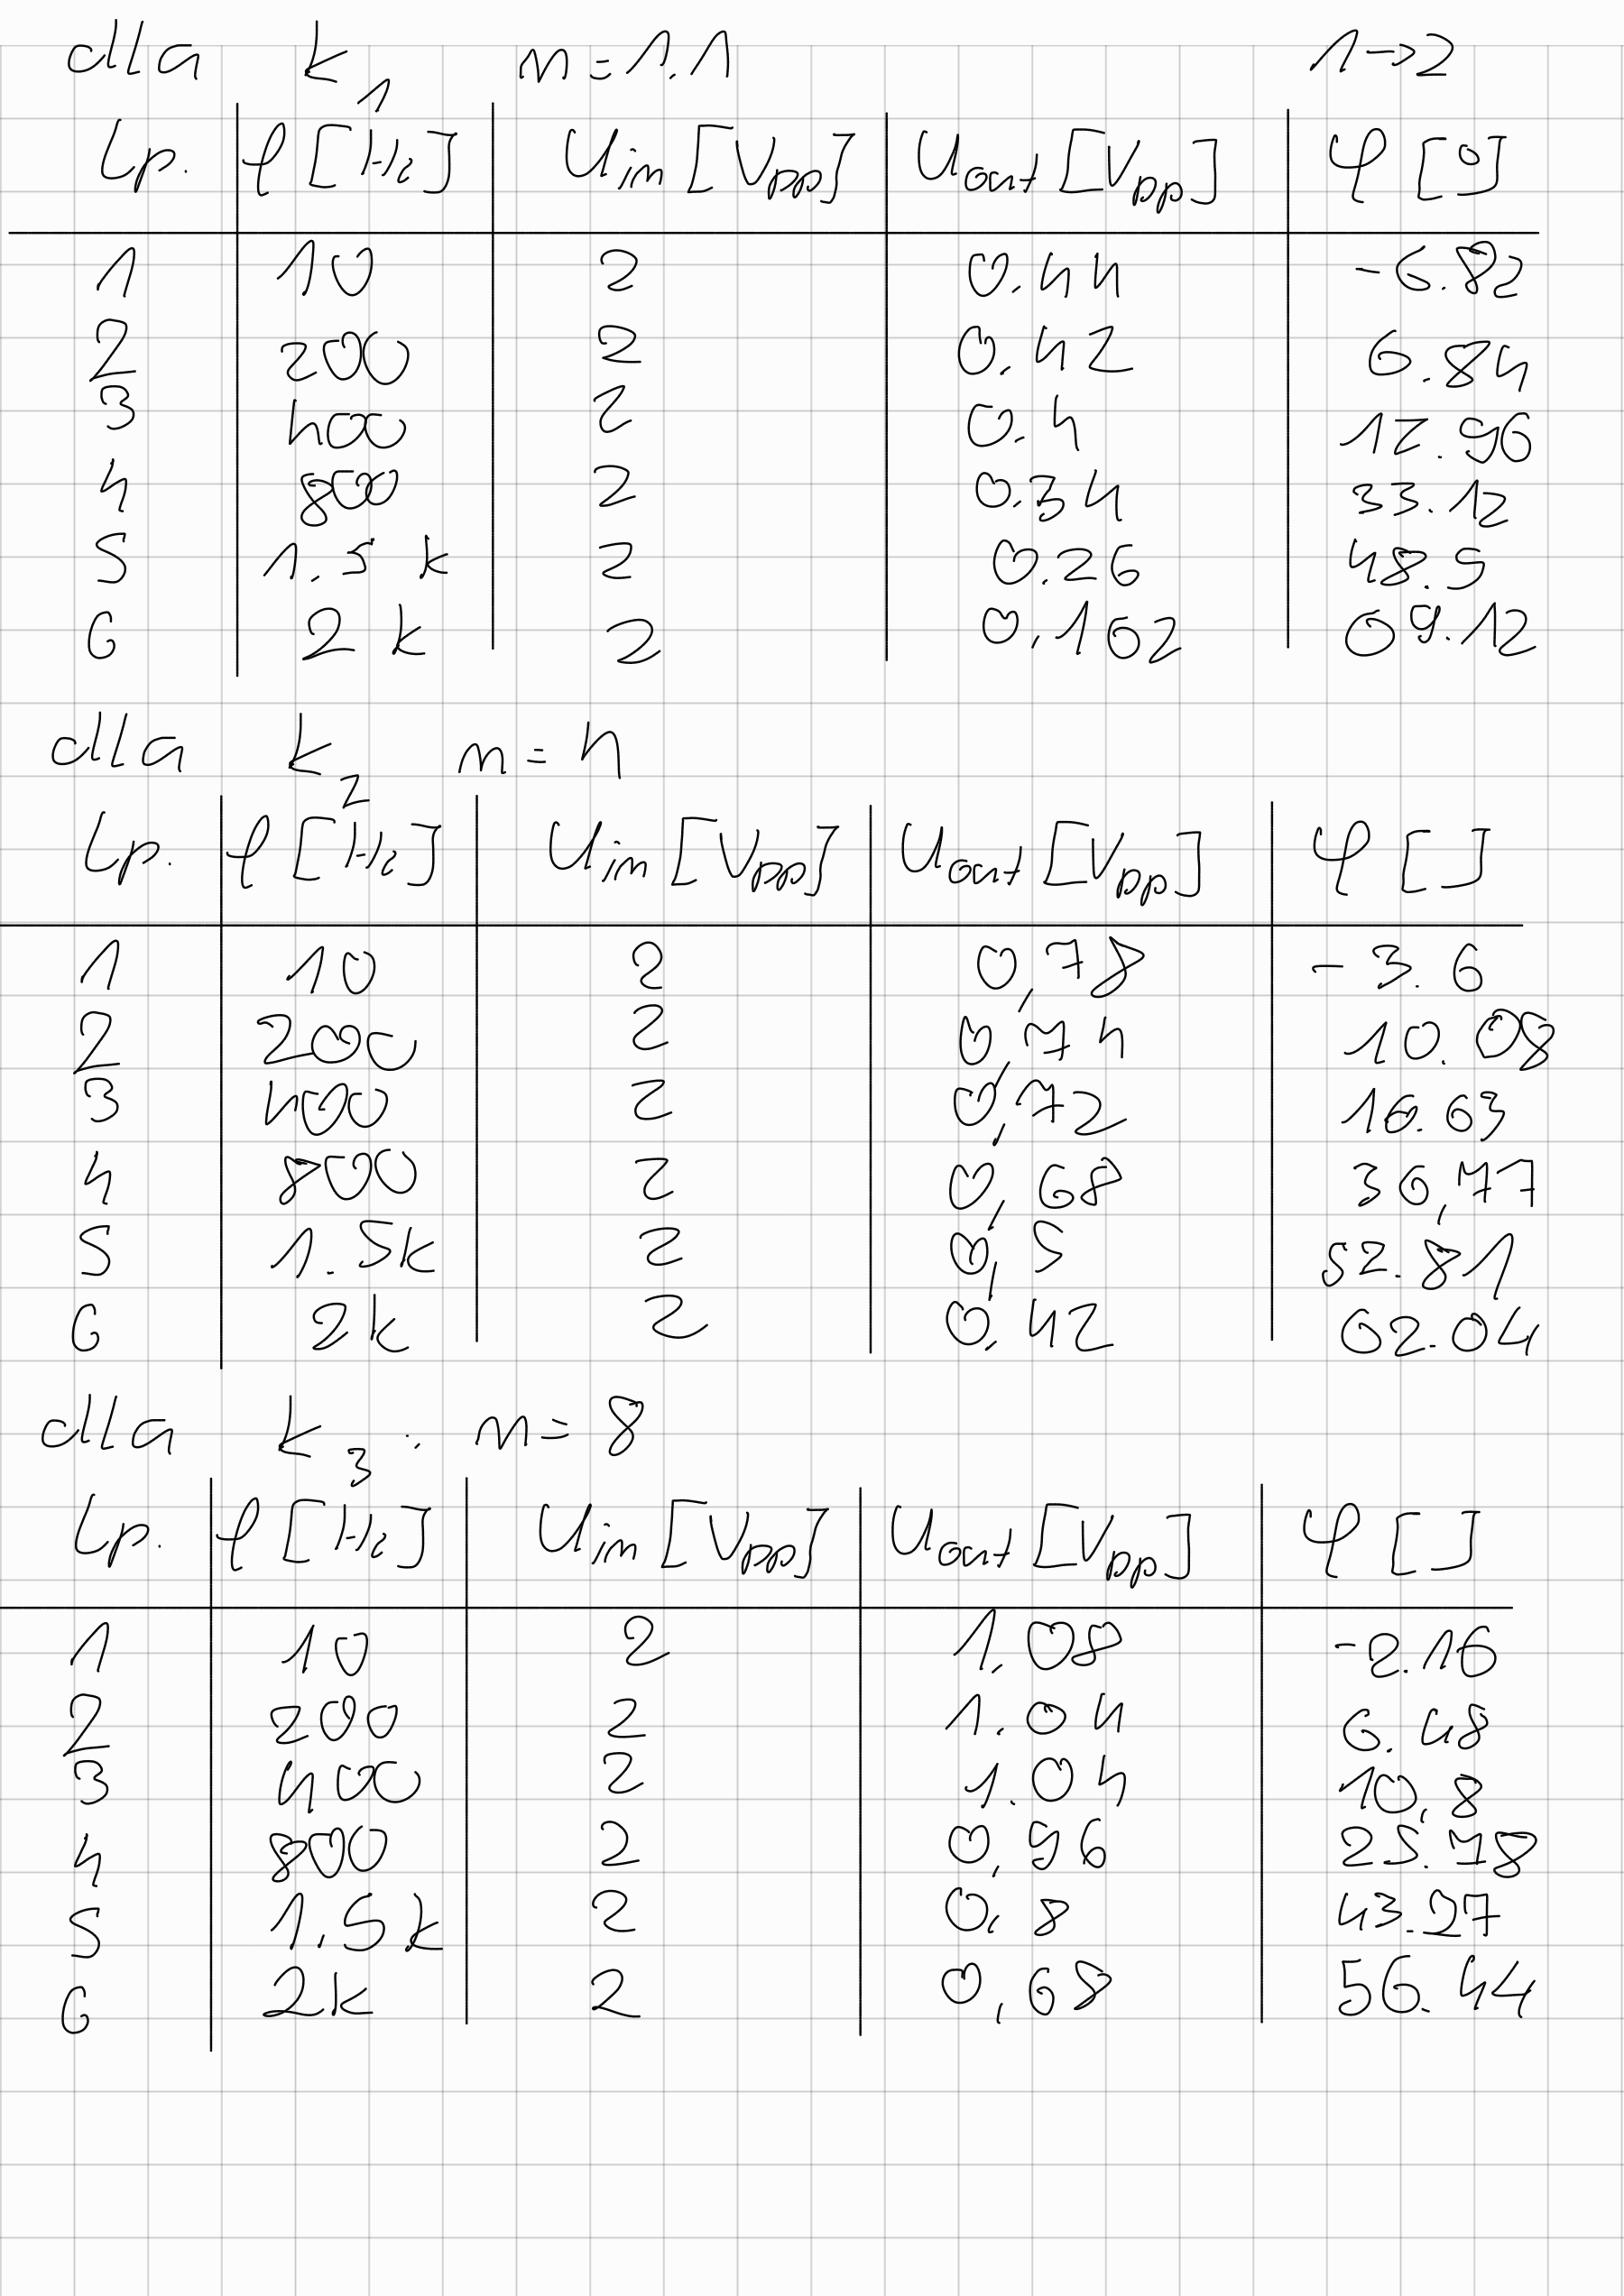
\includegraphics[width=\textwidth]{zdjecia/4.png}
			\caption{Zdjęcie pomiarów 4.}
			\label{fig:pomiar4}
		\end{subfigure}
	\end{figure}
	
	\section{Układy pomiarowe}
	
	Układ A):
	\begin{figure}[H]
		\centering
		\begin{tikzpicture}[
			auto,
			node distance=2.5cm,
			>=Latex,
			block/.style={draw, rectangle, minimum height=1cm, minimum width=2cm},
			sum/.style={draw, circle, node distance=1.5cm},
			gain/.style={draw, regular polygon, regular polygon sides=3, shape border rotate=-90, minimum size=1.2cm, inner sep=0pt}
			]
			% --- Definicja węzłów (elementów schematu) ---
			\node[coordinate] (input) {}; % Punkt startowy dla wejścia
			\node[sum, right=1.5cm of input] (sum) {}; % Węzeł sumacyjny
			\node[gain, right=1.5cm of sum] (gain) {$k_c$}; % Wzmacniacz
			\node[block, right=1.5cm of gain] (integrator) {$\frac{1}{sT_i}$}; % Blok całkujący
			\node[block, right=2cm of integrator] (system) {$\frac{1}{s^2 a_2 + s a_1 + 1}$}; % Blok główny
			\node[coordinate, right=1.5cm of system] (output) {}; % Punkt końcowy dla wyjścia
			
			% --- Rysowanie strzałek i sygnałów ---
			\draw[->] (input) -- node[pos=0.2, above] {$r(t)$} (sum);
			\draw[->] (sum) -- node[above] {$e(t)$} (gain);
			\draw[->] (gain) -- node[above] {$u(t)$} (integrator);
			\draw[->] (integrator) -- (system);
			
			% --- Pętla sprzężenia zwrotnego ---
			% Najpierw rysujemy linię od bloku do punktu rozgałęzienia i dalej do wyjścia
			\draw[-] (system.east) -- ++(0.75,0) coordinate (branch_point);
			\draw[->] (branch_point) -- node[pos=0.5, above] {$c(t)$} (output);
			% Teraz rysujemy pętlę zwrotną od punktu rozgałęzienia do węzła sumacyjnego
			\draw[->] (branch_point) |- ++(0,-2cm) -| node[pos=0.95, right] {$-$} (sum.south);
			
			% --- Etykieta (a) ---
			\node at (output.east) [right=0.5cm] {(a)};
			
		\end{tikzpicture}
		\caption{Schemat układu pomiarowego (a).}
	\end{figure}
	
	\noindent Układ B):
	\begin{figure}[H]
		\centering
		\begin{tikzpicture}[
			auto,
			node distance=2.5cm,
			>=Latex,
			block/.style={draw, rectangle, minimum height=1cm, minimum width=2.5cm, align=center},
			sum/.style={draw, circle, node distance=1.5cm},
			gain/.style={draw, regular polygon, regular polygon sides=3, shape border rotate=-90, minimum size=1.2cm, inner sep=0pt}
			]
			% --- Definicja węzłów (elementów schematu) ---
			\node[coordinate] (input) {}; % Punkt startowy dla wejścia
			\node[sum, right=1.5cm of input] (sum) {}; % Węzeł sumacyjny
			\node[gain, right=1.5cm of sum] (gain) {$k_c$}; % Wzmacniacz
			\node[block, right=1.5cm of gain] (integrator) {$\frac{1}{sT_i}$}; % Blok całkujący
			\node[block, right=2.2cm of integrator] (system) {$\frac{1-sT_x}{1+sT_y}$}; % Blok główny
			\node[coordinate, right=1.5cm of system] (output) {}; % Punkt końcowy dla wyjścia
			
			% --- Rysowanie strzałek i sygnałów ---
			\draw[->] (input) -- node[pos=0.2, above] {$r(t)$} (sum);
			\draw[->] (sum) -- node[above] {$e(t)$} (gain);
			\draw[->] (gain) -- node[above] {$u(t)$} (integrator);
			\draw[->] (integrator) -- (system);
			
			% --- Pętla sprzężenia zwrotnego ---
			% Rysowanie linii od bloku do punktu rozgałęzienia i dalej do wyjścia
			\draw[-] (system.east) -- ++(0.75,0) coordinate (branch_point);
			\draw[->] (branch_point) -- node[pos=0.5, above] {$c(t)$} (output);
			% Rysowanie pętli zwrotnej
			\draw[->] (branch_point) |- ++(0,-2cm) -| node[pos=0.95, right] {$-$} (sum.south);
			
		\end{tikzpicture}
		\caption{Schemat układu pomiarowego (b).}
	\end{figure}
	
	\noindent Układ D):
	\begin{figure}[H]
		\centering
		\begin{tikzpicture}[
			auto,
			node distance=2.5cm,
			>=Latex,
			block/.style={draw, rectangle, minimum height=1cm, minimum width=2.5cm, align=center},
			sum/.style={draw, circle, node distance=1.5cm},
			gain/.style={draw, regular polygon, regular polygon sides=3, shape border rotate=-90, minimum size=1.2cm, inner sep=0pt}
			]
			% --- Definicja węzłów (elementów schematu) ---
			\node[coordinate] (input) {};
			\node[sum, right=1.5cm of input] (sum1) {};
			\node[gain, right=1.5cm of sum1] (gain) {$k_c$};
			\node[sum, right=1.5cm of gain] (sum2) {};
			\node[block, right=1.5cm of sum2] (system) {$\frac{k_p}{sT_p+1}$};
			\node[coordinate, right=1.5cm of system] (output) {};
			
			% --- Rysowanie strzałek i sygnałów (ścieżka główna) ---
			\draw[->] (input) -- node[pos=0.2, above] {$r(t)$} (sum1);
			\draw[->] (sum1) -- node[above] {$e(t)$} (gain);
			\draw[->] (gain) -- node[above] {$u(t)$} (sum2);
			\draw[->] (sum2) -- node[above] {$a(t)$} (system);
			
			% --- Dodanie zakłócenia d(t) ---
			\draw[->] (sum2.north) ++(0,1.2cm) node[above] {$d(t)$} -- node[pos=0.4, right] {$+$} (sum2);
			
			% --- Pętla sprzężenia zwrotnego i wyjście ---
			\draw[-] (system.east) -- ++(0.75,0) coordinate (branch_point);
			\draw[->] (branch_point) -- node[pos=0.5, above] {$c(t)$} (output);
			\draw[->] (branch_point) |- ++(0,-2cm) -| node[pos=0.95, right] {$-$} (sum1.south);
			
		\end{tikzpicture}
		\caption{Schemat blokowy układu regulacji z zakłóceniem.}
	\end{figure}	
	
	\newpage
	\section{Układ A}
	
	Pierwszy badany układ składa się ze sterownika proporcjonalnego (P) oraz obiektu sterowanego w pętli ujemnego sprzężenia zwrotnego. Obiekt sterowany jest szeregowym połączeniem członu całkującego i członu inercyjnego drugiego rzędu. 
	
	Na podstawie identyfikacji przeprowadzonej w ćwiczeniu 1, przyjęto następujące parametry modeli:
	\begin{itemize}
		\item Człon całkujący: $G(s) = \frac{1}{sT_i}$, gdzie $T_i = 1,33 \text{ ms}$.
		\item Człon 2 rzędu: $G(s) = \frac{1}{1 + sa_1 + s^2a_2} = \frac{1}{1+s 2\zeta \tau + s^2 \tau^2} = \frac{w_n^2}{w_n^2 + s 2 \zeta w_n + s^2}$, gdzie wyznaczone parametry to $\zeta = 0,336$ i $\omega_n = 2560 \text{ rad/s}$.
	\end{itemize}
	
	Badania przeprowadzono dla trzech różnych wartości wzmocnienia \(k_c\), obliczonych ze wzoru \(k_c = 0,47 + n/2\):
	\begin{itemize}
		\item Dla \(n_1 = 0,1\): $k_{c1} = 0,47 + 0,1 / 2 = 0,47 + 0,05 = \textbf{0,52}$
		\item Dla \(n_2 = 1,3\): $k_{c2} = 0,47 + 1,3 / 2 = 0,47 + 0,65 = \textbf{1,12}$
		\item Dla \(n_3 = 2,4\): $k_{c3} = 0,47 + 2,4 / 2 = 0,47 + 1,20 = \textbf{1,67}$
	\end{itemize}
	
	\subsection{Odpowiedzi skokowe}
	Na poniższym wykresie przedstawiono zarejestrowane odpowiedzi skokowe układu (A) dla trzech wyznaczonych wzmocnień \(k_c\).
	
	\begin{figure}[H]
		\centering
		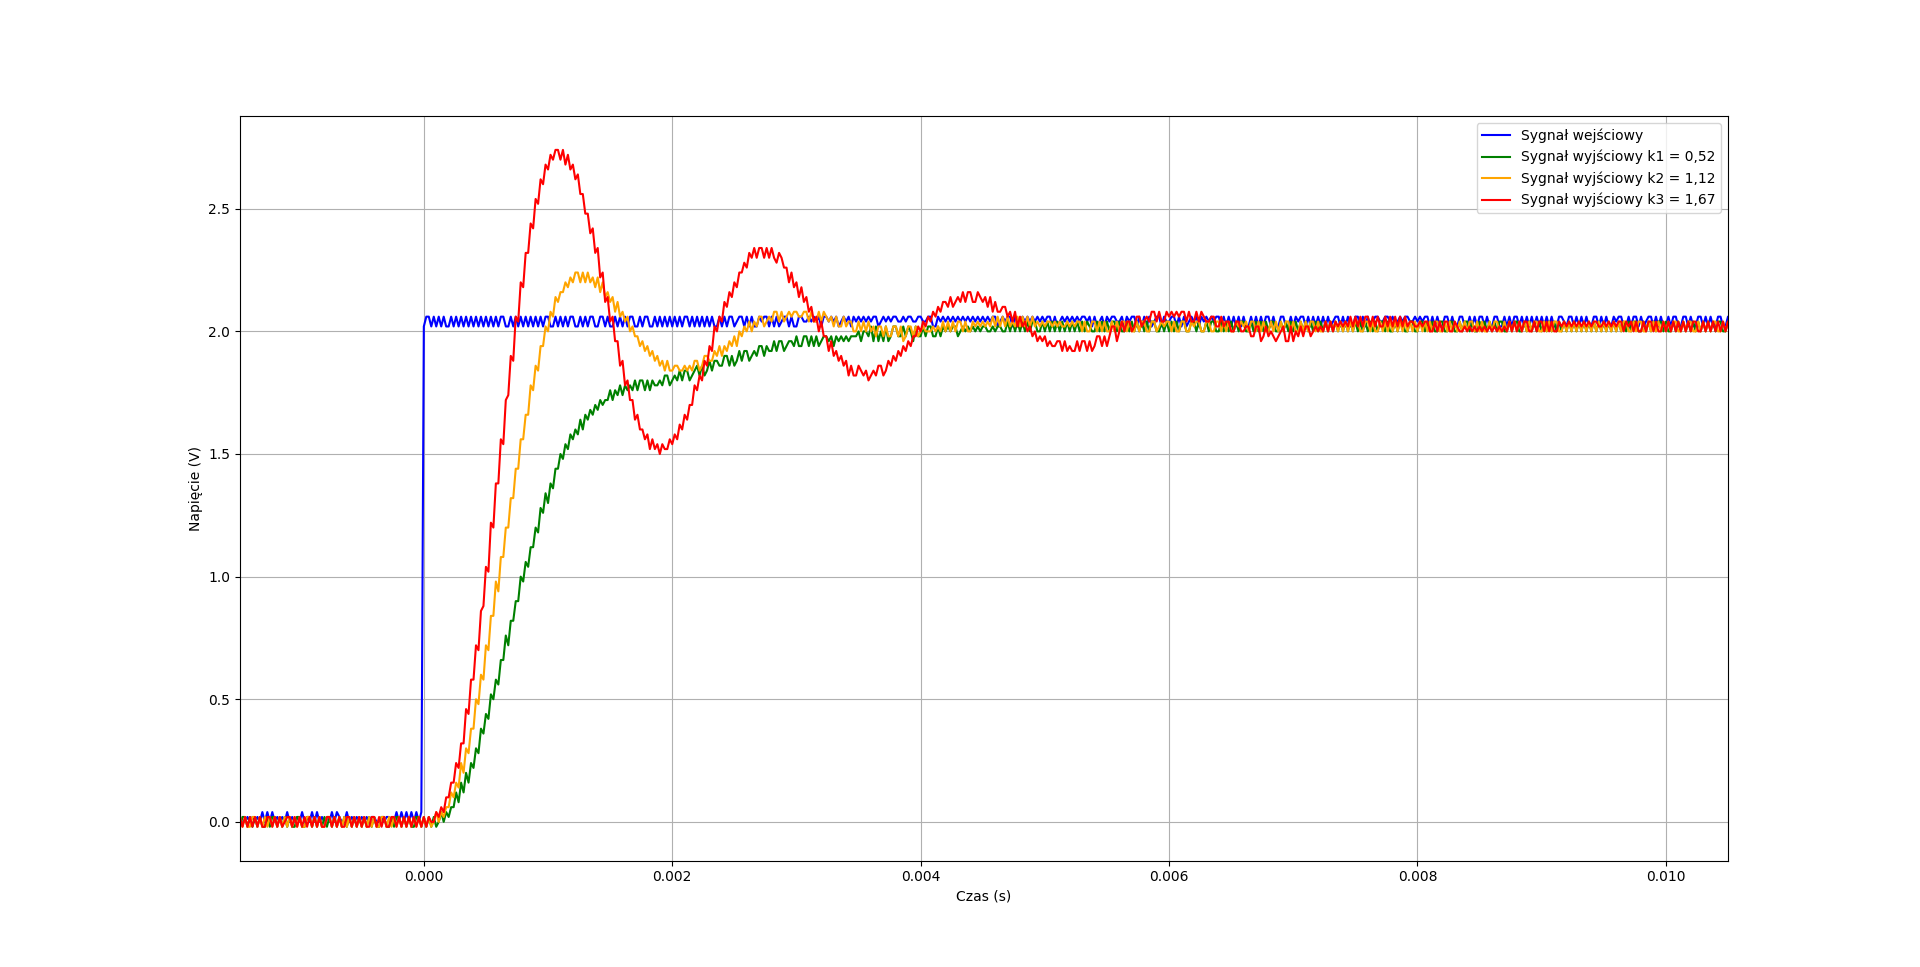
\includegraphics[width=1\linewidth]{zdjecia/OdpSkokA.png}
		\caption{Odpowiedź skokowa układu (A) przy różnych wartościach wzmocnienia \(k_c\) wykreślona z pliku CSV.}
		\label{fig:OdpSkokA}
	\end{figure}
	
	Analiza odpowiedzi skokowych Układu A pokazuje, że zwiększanie wzmocnienia $k_c$ skraca czas narastania, ale jednocześnie znacząco zwiększa przeregulowanie i oscylacyjność odpowiedzi. Niezależnie od wzmocnienia, uchyb ustalony wynosi zero, co jest zasługą członu całkującego w obiekcie sterowania.
	
	\subsection{Linie pierwiastkowe}
	Wykres linii pierwiastkowych dla układu otwartego \(G_o(s) = k_c \cdot \frac{1}{sT_i} \cdot \frac{w_n^2}{w_n^2 + s 2 \zeta w_n + s^2}\) przedstawiono poniżej. Zaznaczono na nim położenie biegunów układu zamkniętego dla badanych wzmocnień \(k_{c1}\), \(k_{c2}\) i \(k_{c3}\).
	
	\begin{figure}[H]
		\centering
		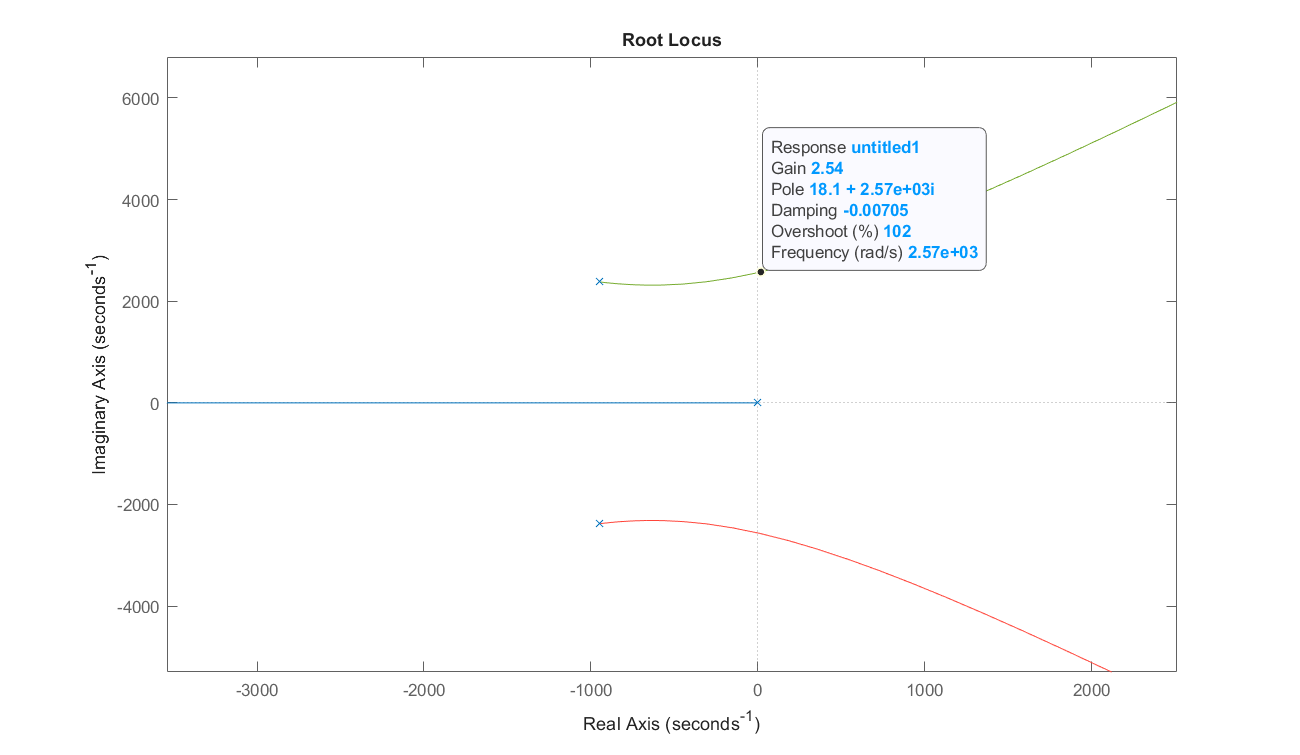
\includegraphics[width=0.8\linewidth]{zdjecia/LP_ukladA.png}
		\caption{Linie pierwiastkowe układu otwartego (A).}
		\label{fig:LP_ukladA}
	\end{figure}
	
	Wykres linii pierwiastkowych pokazuje, że wraz ze wzrostem $k_c$ bieguny układu zamkniętego zbliżają się do osi urojonej. Powoduje to spadek tłumienia, co bezpośrednio przekłada się na większe oscylacje widoczne na odpowiedziach skokowych. Linie pierwiastkowe wskazują również, że zbyt duże wzmocnienie $k_c$ doprowadzi do niestabilności systemu, ponieważ gałęzie zmierzają w kierunku prawej półpłaszczyzny. 
	
	\subsection{Charakterystyki Bodego}
	Poniższy wykres przedstawia charakterystyki Bodego układu zamkniętego dla badanych wartości \(k_c\).
	
	\begin{figure}[H]
		\centering
		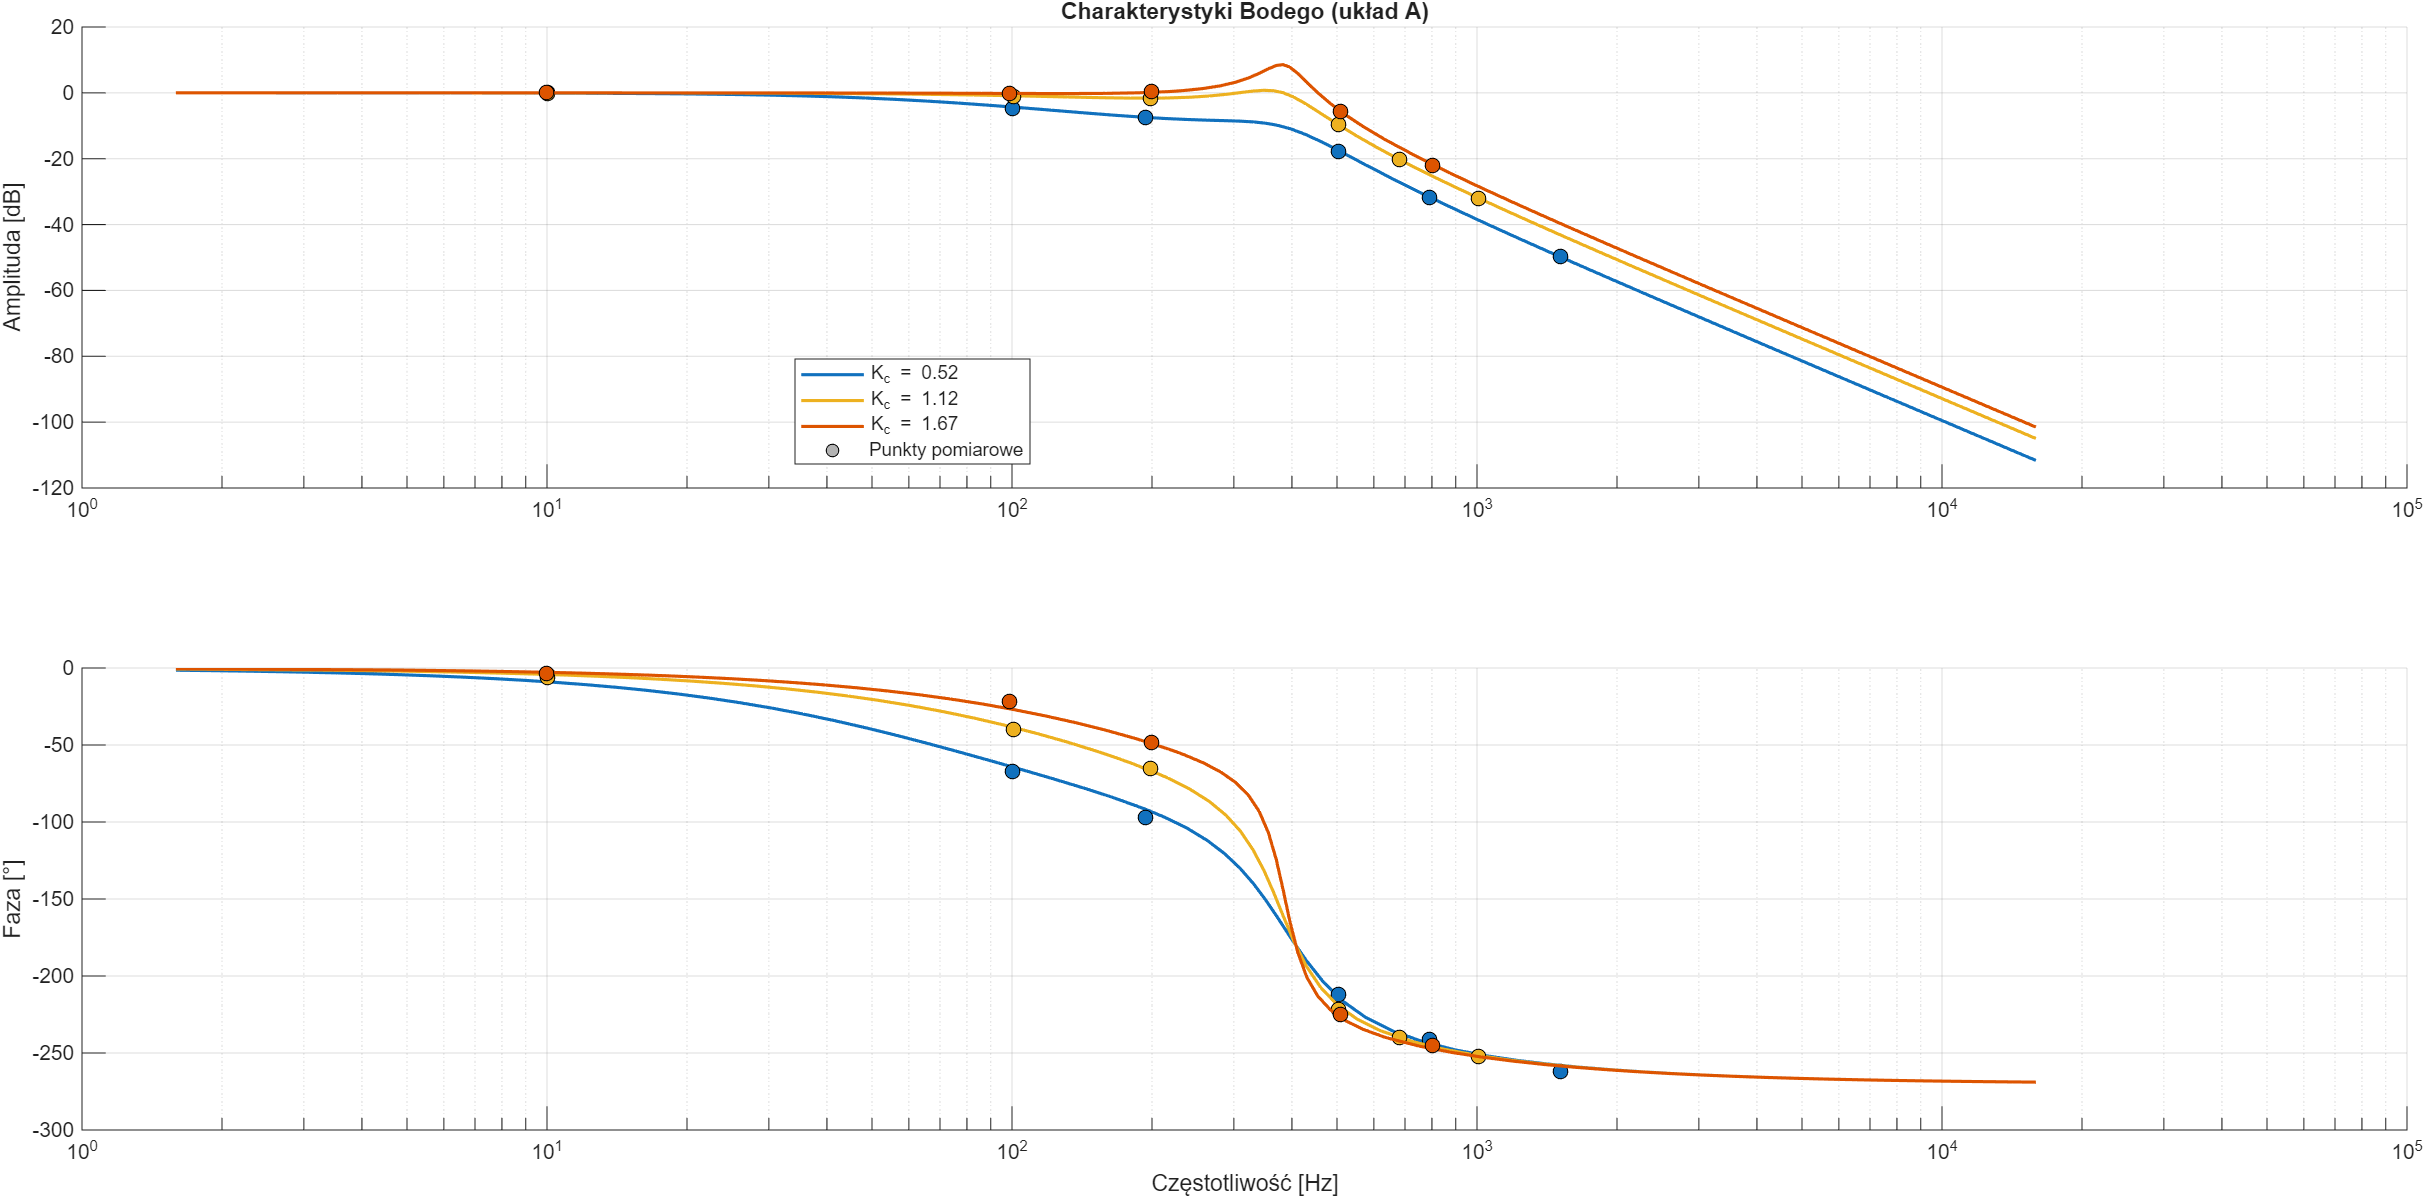
\includegraphics[width=1\linewidth]{zdjecia/Bode_ukladA.png}
		\caption{Charakterystyki Bodego układu zamkniętego (A).}
		\label{fig:Bode_ukladA}
	\end{figure}
	
	Charakterystyki Bodego układu zamkniętego (Rysunek 7) pokazują, jak wzmocnienie $k_c$ wpływa na odpowiedź częstotliwościową. Wzrost $k_c$ powoduje pojawienie się i wzrost piku rezonansowego, oraz lekkie poszerzenie pasma przenoszenia. Wyższy pik rezonansowy jest bezpośrednio skorelowany z mniejszym tłumieniem i większym przeregulowaniem, co jest w pełni zgodne z analizą odpowiedzi skokowych (Rysunek 5).
	
	\subsection{Charakterystyki Nyquista}
	Na wykresie Nyquista układu otwartego można zbadać stabilność układu zamkniętego.
	
	\begin{figure}[H]
		\centering
		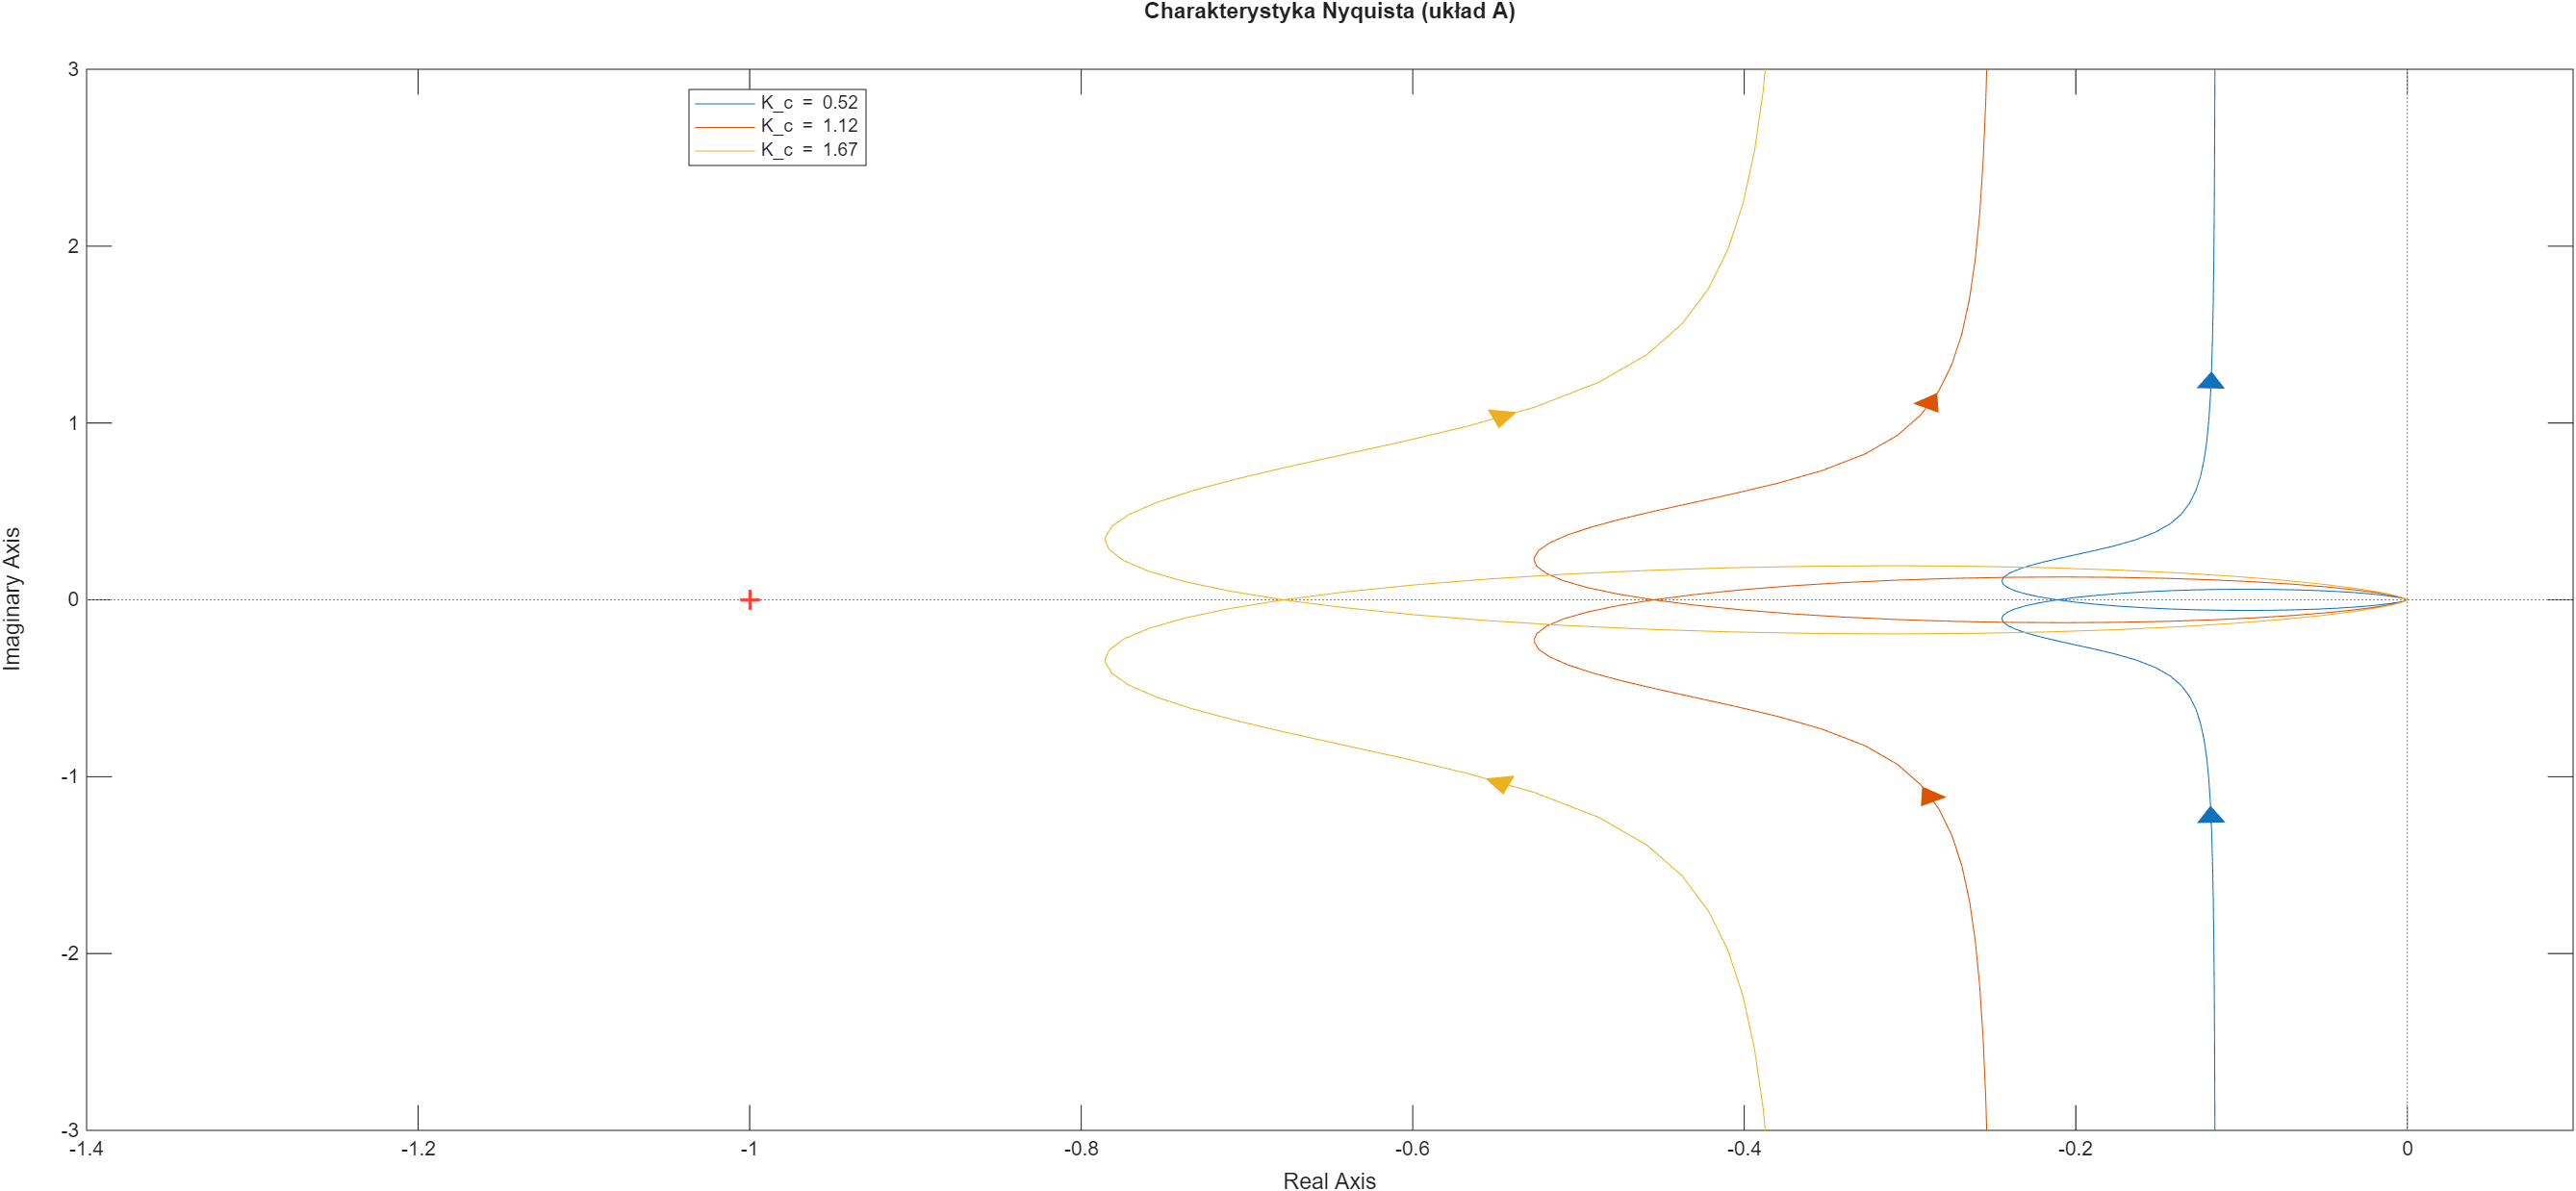
\includegraphics[width=0.8\linewidth]{zdjecia/NQ_ukladA.png}
		\caption{Charakterystyka Nyquista układu otwartego (A).}
		\label{fig:NQ_ukladA}
	\end{figure}

	Wykres Nyquist układu otwartego (Rysunek 8) służy do oceny stabilności układu zamkniętego. Wzrost $k_c$ powoduje proporcjonalne skalowanie wykresu. Dla małego wzmocnienia ($k_{c1}=0.52$), wykres jest daleko od punktu krytycznego (-1, 0j), co oznacza duży zapas stabilności. W miarę wzrostu $k_c$ do 1.67, wykres niebezpiecznie zbliża się do punktu (-1, 0j), co sygnalizuje mały zapas fazy i wzmocnienia oraz, co za tym idzie, silne oscylacje widoczne na odpowiedzi skokowej.
	
	\subsection{Analityczne uzasadnienie wyników dla układu A (Obiekt całkująco-inercyjny II rzędu)}
	
	\textbf{Model obiektu:} $G_p(s) = \frac{1}{sT_i} \cdot \frac{\omega_n^2}{s^2 + 2\zeta\omega_n s + \omega_n^2}$. \\
	\textbf{Transmitancja układu otwartego:} $G_o(s) = k_c \cdot G_p(s) = \frac{k_c \omega_n^2}{sT_i(s^2 + 2\zeta\omega_n s + \omega_n^2)}$.
	
	\subsubsection{Dokładność sterowania (Uchyb ustalony)}
	\begin{itemize}
		\item \textbf{Uzasadnienie analityczne:} Układ otwarty $G_o(s)$ posiada biegun w początku układu współrzędnych (człon całkujący $1/sT_i$). Czyni to system \textbf{układem typu 1}. Zgodnie z twierdzeniem o wartości końcowej, uchyb ustalony $e$ dla pobudzenia skokowego $R(s) = 1/s$ wynosi:
		\[
		e = \lim_{s \to 0} s \cdot E(s) = \lim_{s \to 0} s \cdot \frac{R(s)}{1 + G_o(s)} = \lim_{s \to 0} \frac{1}{1 + G_o(s)}
		\]
		\[
		e = \lim_{s \to 0} \frac{1}{1 + \frac{k_c \omega_n^2}{sT_i(s^2 + 2\zeta\omega_n s + \omega_n^2)}} = \frac{1}{1 + \infty} = 0
		\]
		\item \textbf{Zgodność z pomiarami:} Analiza potwierdza obserwacje pomiarowe (Rysunek \ref{fig:OdpSkokA}), że \textbf{uchyb ustalony wynosi zero niezależnie od wartości $k_c$}. Jest to bezpośrednia konsekwencja obecności członu całkującego w obiekcie.
	\end{itemize}
	
	\subsubsection{Jakość odpowiedzi skokowej i stabilność}
	\begin{itemize}
		\item \textbf{Uzasadnienie analityczne:} Transmitancja układu zamkniętego $G_z(s) = \frac{G_o(s)}{1 + G_o(s)}$ posiada równanie charakterystyczne:
		\[
		1 + G_o(s) = 0 \implies sT_i(s^2 + 2\zeta\omega_n s + \omega_n^2) + k_c \omega_n^2 = 0
		\]
		\[
		s^3 T_i + 2\zeta\omega_n T_i s^2 + \omega_n^2 T_i s + k_c \omega_n^2 = 0
		\]
		Jest to układ \textbf{trzeciego rzędu}. Stabilność takiego układu można zbadać kryterium Routha-Hurwitza. Warunkiem stabilności (poza dodatniością współczynników $T_i, 2\zeta\omega_n T_i, \omega_n^2 T_i, k_c \omega_n^2 > 0$) jest:
		\[
		(2\zeta\omega_n T_i) \cdot (\omega_n^2 T_i) > (T_i) \cdot (k_c \omega_n^2)
		\]
		\[
		2\zeta\omega_n T_i^2 \omega_n^2 > k_c T_i \omega_n^2 \implies 2\zeta\omega_n T_i > k_c
		\]
		Istnieje więc wzmocnienie graniczne $k_{gr} = 2\zeta\omega_n T_i$, powyżej którego układ staje się niestabilny. Wzrost $k_c$ przesuwa bieguny dominujące układu zamkniętego w kierunku osi urojonej $j\omega$.
		
		\item \textbf{Zgodność z pomiarami:} Model analityczny w pełni tłumaczy wyniki pomiarów. Jak widać na Rysunku \ref{fig:OdpSkokA}, zwiększanie $k_c$ \textbf{skraca czas narastania, ale jednocześnie zwiększa przeregulowanie i oscylacyjność}. Dzieje się tak, ponieważ bieguny zbliżają się do osi $j\omega$ (co widać na Rysunku \ref{fig:LP_ukladA}), zmniejszając tłumienie systemu. Wykres Nyquista (Rysunek \ref{fig:NQ_ukladA}), skalowany przez $k_c$, potwierdza, że dla większych wzmocnień pętla $G_o(j\omega)$ zbliża się do punktu krytycznego (-1, 0j), co sygnalizuje spadek zapasu fazy i wzmocnienia oraz wzrost oscylacji.
	\end{itemize}
	
	\subsection{Wpływ wzmocnienia sterownika typu P na postać wszystkich procesów przejściowych w układzie A}
	\begin{itemize}
		\item Sygnał wyjściowy $c(t)$: Zwiększanie wzmocnienia $k_c$ skraca czas narastania odpowiedzi. Jednocześnie jednak, układ staje się bardziej oscylacyjny – rośnie zarówno przeregulowanie, jak i czas ustalania (z powodu dłuższego tłumienia oscylacji). Analiza linii pierwiastkowych potwierdziła, że wzrost $k_c$ przesuwa bieguny układu zamkniętego bliżej osi urojonej, co powoduje spadek tłumienia.
		\item Uchyb $e(t)$: Wzrost $k_c$ powoduje, że uchyb szybciej maleje do zera, ale robi to w sposób bardziej oscylacyjny, z większym przeregulowaniem w kierunku wartości ujemnych. Należy zaznaczyć, że dzięki obecności członu całkującego w obiekcie, uchyb ustalony zawsze dąży do zera, niezależnie od wartości $k_c$.
		\item Sygnał sterujący $u(t)$: Dla skokowej zmiany $r(t)$, uchyb początkowy $e(0)$ jest stały. Wzrost $k_c$ powoduje więc proporcjonalnie większą początkową wartość sygnału sterującego $u(0)$. Ta silniejsza, bardziej agresywna reakcja sterownika jest przyczyną skrócenia czasu narastania. W trakcie stanu przejściowego, oscylacje obecne w $e(t)$ są wzmacniane przez $k_c$, co skutkuje również silnie oscylacyjnym sygnałem $u(t)$.
	\end{itemize}
	
	\bigskip \hrule \bigskip
	
	\section{Układ B}
	
	Drugi badany układ składa się ze sterownika proporcjonalnego (P) oraz obiektu będącego szeregowym połączeniem członu całkującego i członu nieminimalnofazowego.
	
	Na podstawie identyfikacji przeprowadzonej w ćwiczeniu 1, przyjęto następujące parametry modeli:
	\begin{itemize}
		\item Człon całkujący: $G(s) = \frac{1}{sT_i}$, gdzie $T_i = 1,33 \text{ ms}$.
		\item Człon nieminimalnofazowy: $G(s) = \frac{1-sT_x}{1+sT_y}$, gdzie: $T_x = 0,396 \text{ ms}$ i $T_y = 0,113 \text{ ms}$.
	\end{itemize}
	
	Badania przeprowadzono dla trzech wartości wzmocnienia \(k_c\), obliczonych ze wzoru \(k_c = 0,47 + n/2\):
	\begin{itemize}
		\item Dla \(n_1 = 0,5\): $k_{c1} = 0,47 + 0,5 / 2 = 0,47 + 0,25 = \textbf{0,72}$
		\item Dla \(n_2 = 1,5\): $k_{c2} = 0,47 + 1,5 / 2 = 0,47 + 0,75 = \textbf{1,22}$
		\item Dla \(n_3 = 2,8\): $k_{c3} = 0,47 + 2,8 / 2 = 0,47 + 1,40 = \textbf{1,87}$
	\end{itemize}
	
	\subsection{Odpowiedzi skokowe}
	Na poniższym wykresie przedstawiono zarejestrowane odpowiedzi skokowe układu (B) dla trzech wyznaczonych wzmocnień \(k_c\).
	
	\begin{figure}[H]
	\centering
	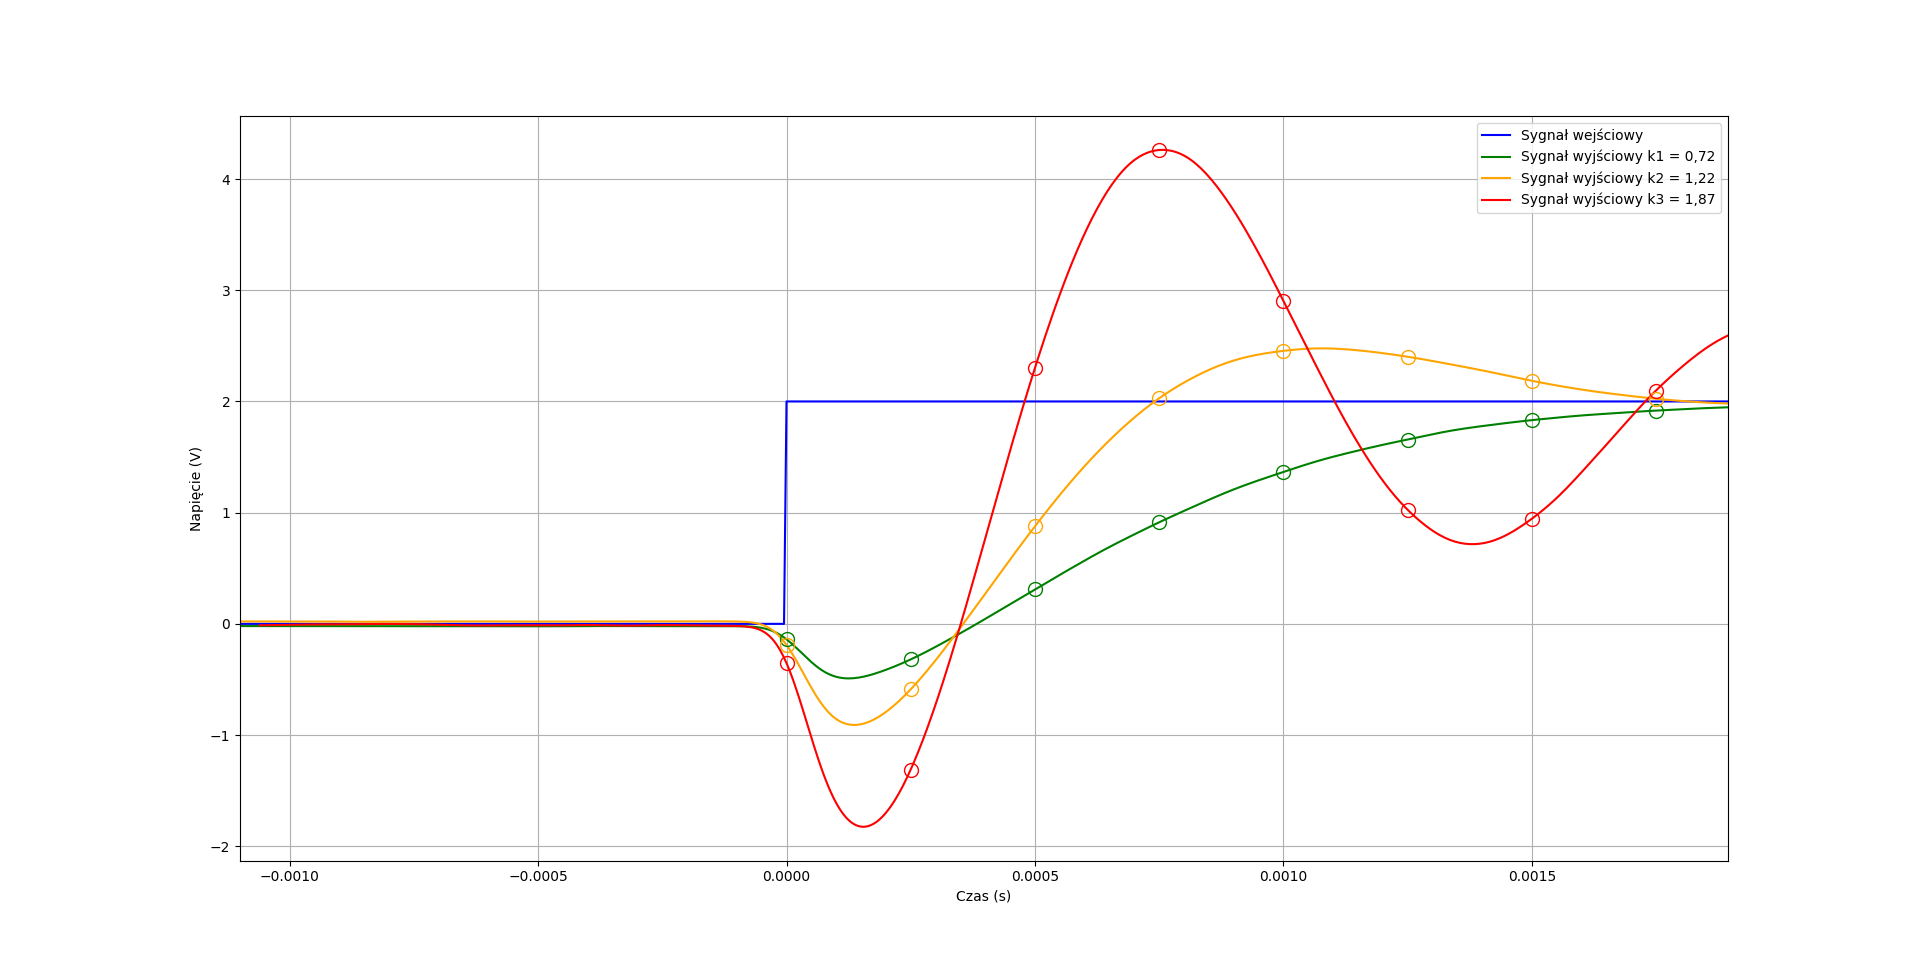
\includegraphics[width=1\linewidth]{zdjecia/OdpSkokB.png}
	\caption{Odpowiedź skokowa układu (B) przy różnych wartościach wzmocnienia \(k_c\).}
	\label{fig:OdpSkokB}
	\end{figure}
	
	Odpowiedzi skokowe Układu B (Rys. 9) wykazują cechy charakterystyczne dla układu nieminimalnofazowego, co jest zgodne z jego modelem. Kluczowym elementem jest sygnał wyjściowy, który początkowo podąża w kierunku przeciwnym do wartości zadanej. Wzrost wzmocnienia $k_c$ skraca czas narastania, ale jednocześnie drastycznie pogłębia początkowe zanurkowanie oraz zwiększa przeregulowanie i oscylacyjność. Dla $k_{c3}=1.87$ układ jest już na granicy stabilności. Podobnie jak w Układzie A, obecność członu całkującego zapewnia zerowy uchyb ustalony.
	
	\subsection{Linie pierwiastkowe}
	Wykres linii pierwiastkowych dla układu otwartego \(G_o(s) = k_c \cdot \frac{1}{sT_i} \cdot
	\frac{1-sT_x}{1+sT_y}\) przedstawiono poniżej. Zaznaczono na nim położenie biegunów układu zamkniętego dla badanych wzmocnień \(k_{c1}\), \(k_{c2}\) i \(k_{c3}\).
	
	\begin{figure}[H]
		\centering
		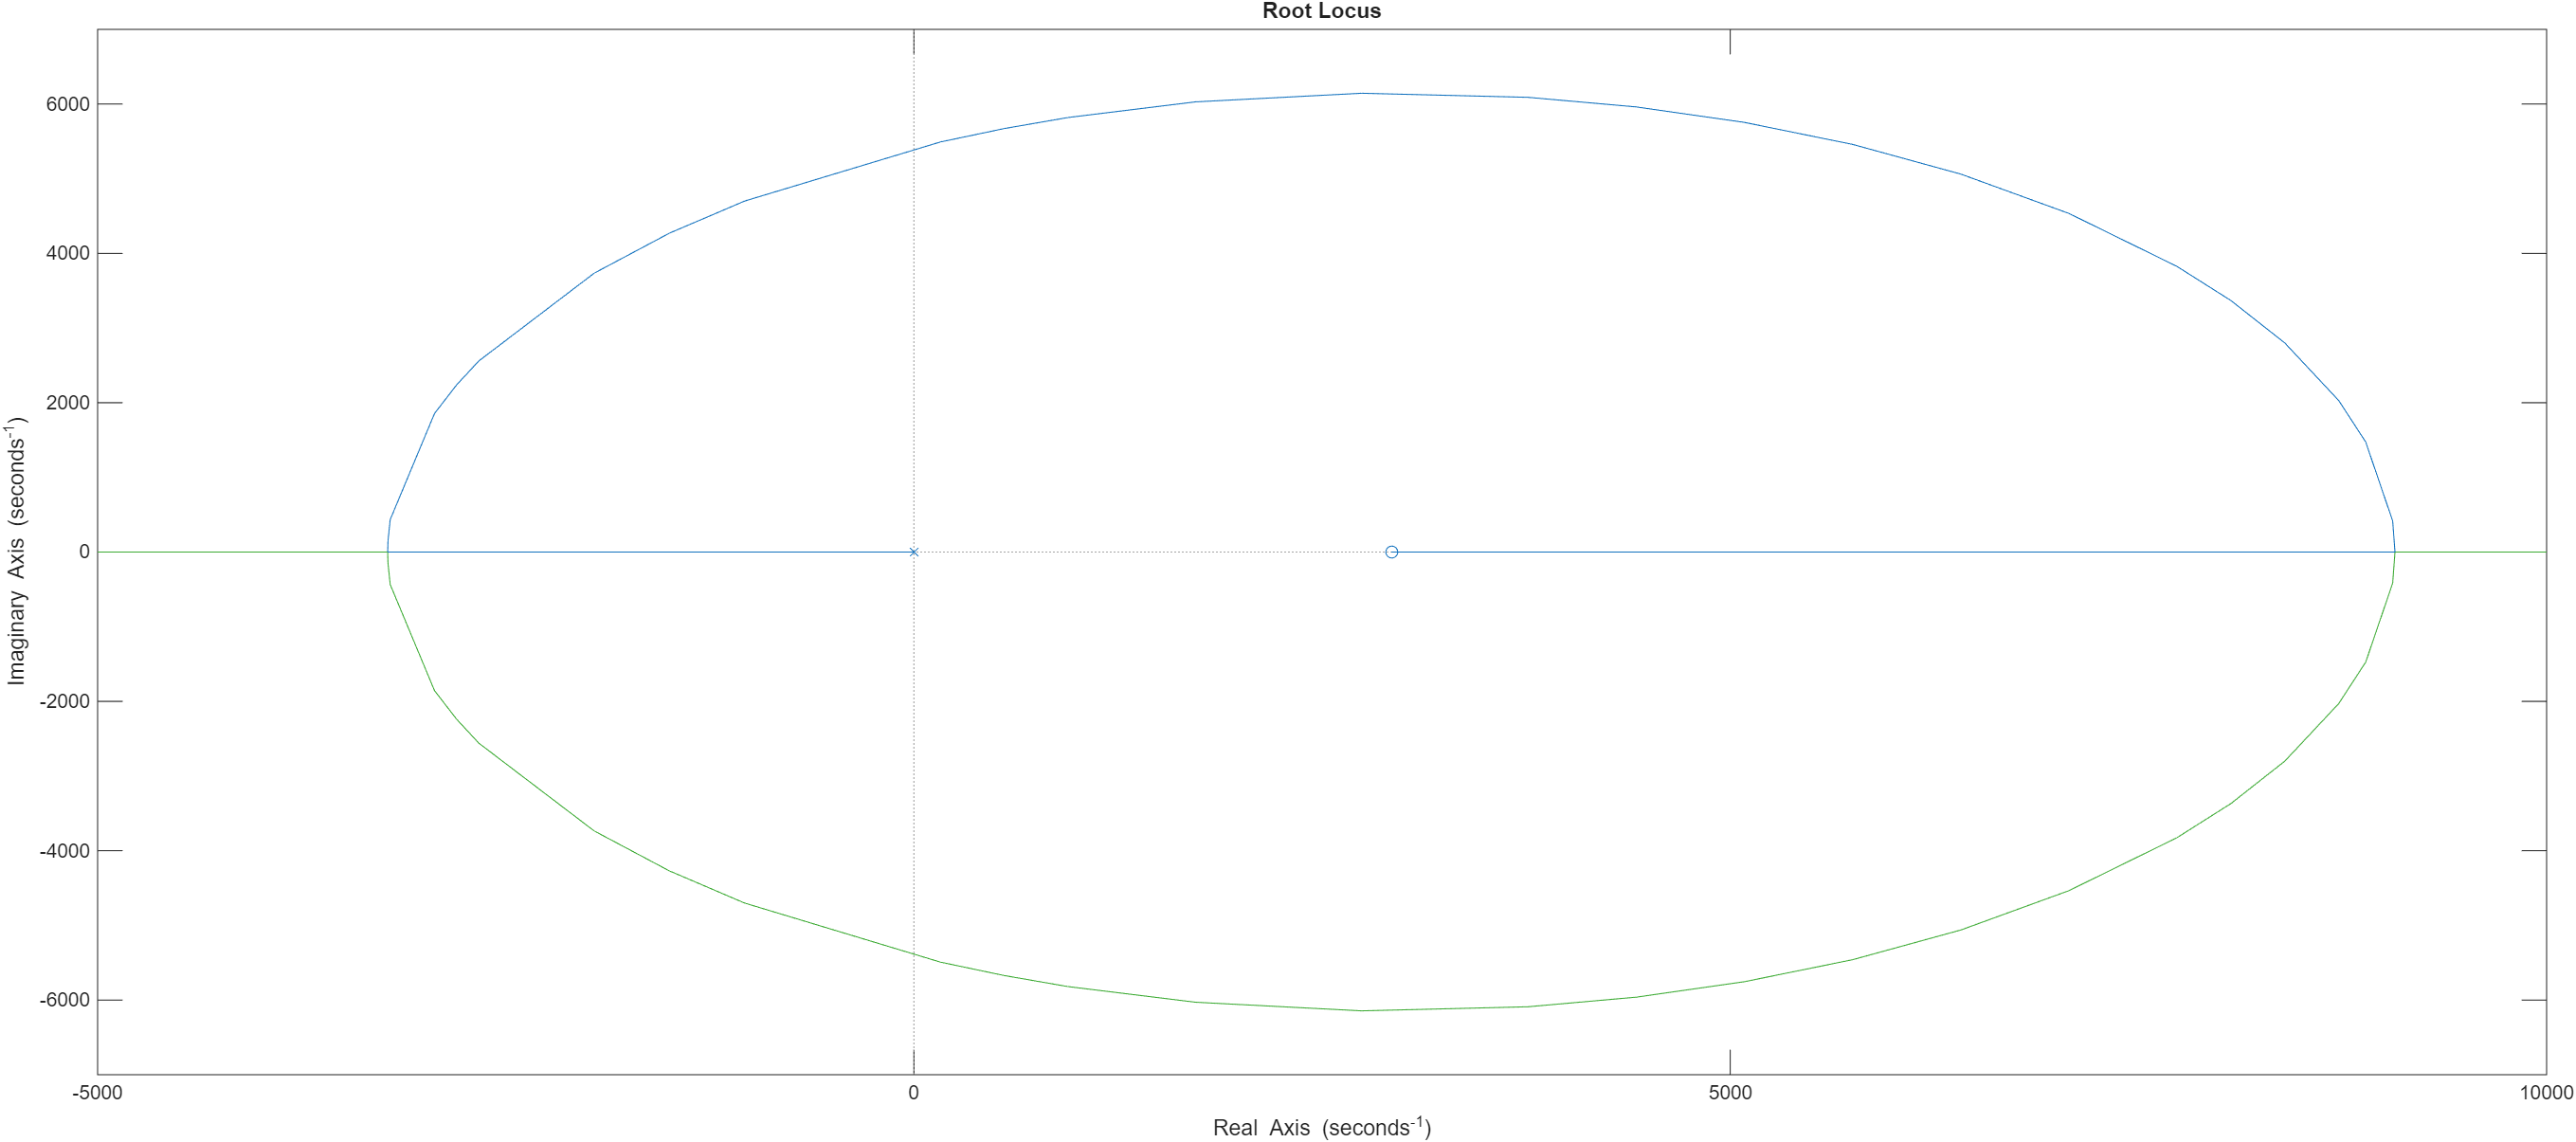
\includegraphics[width=0.8\linewidth]{zdjecia/LP_ukladB.png}
		\caption{Linie pierwiastkowe układu otwartego (B).}
		\label{fig:LP_ukladB}
	\end{figure}
	
	Wykres linii pierwiastkowych dla Układu B (Rys. 10) jest zdominowany przez obecność zera w prawej półpłaszczyźnie (wynikającego z członu nieminimalnofazowego). To zero przyciąga do siebie jedną z gałęzi linii pierwiastkowych, powodując, że bieguny układu zamkniętego bardzo szybko przekraczają oś urojoną i przechodzą do strefy niestabilnej. Wyjaśnia to, dlaczego już stosunkowo niewielki wzrost $k_c$ prowadzi do tak silnych oscylacji i szybkiej utraty stabilności, co zaobserwowano na odpowiedzi skokowej (Rys. 9).
	
	\subsection{Charakterystyki Bodego}
	
	\begin{figure}[H]
		\centering
		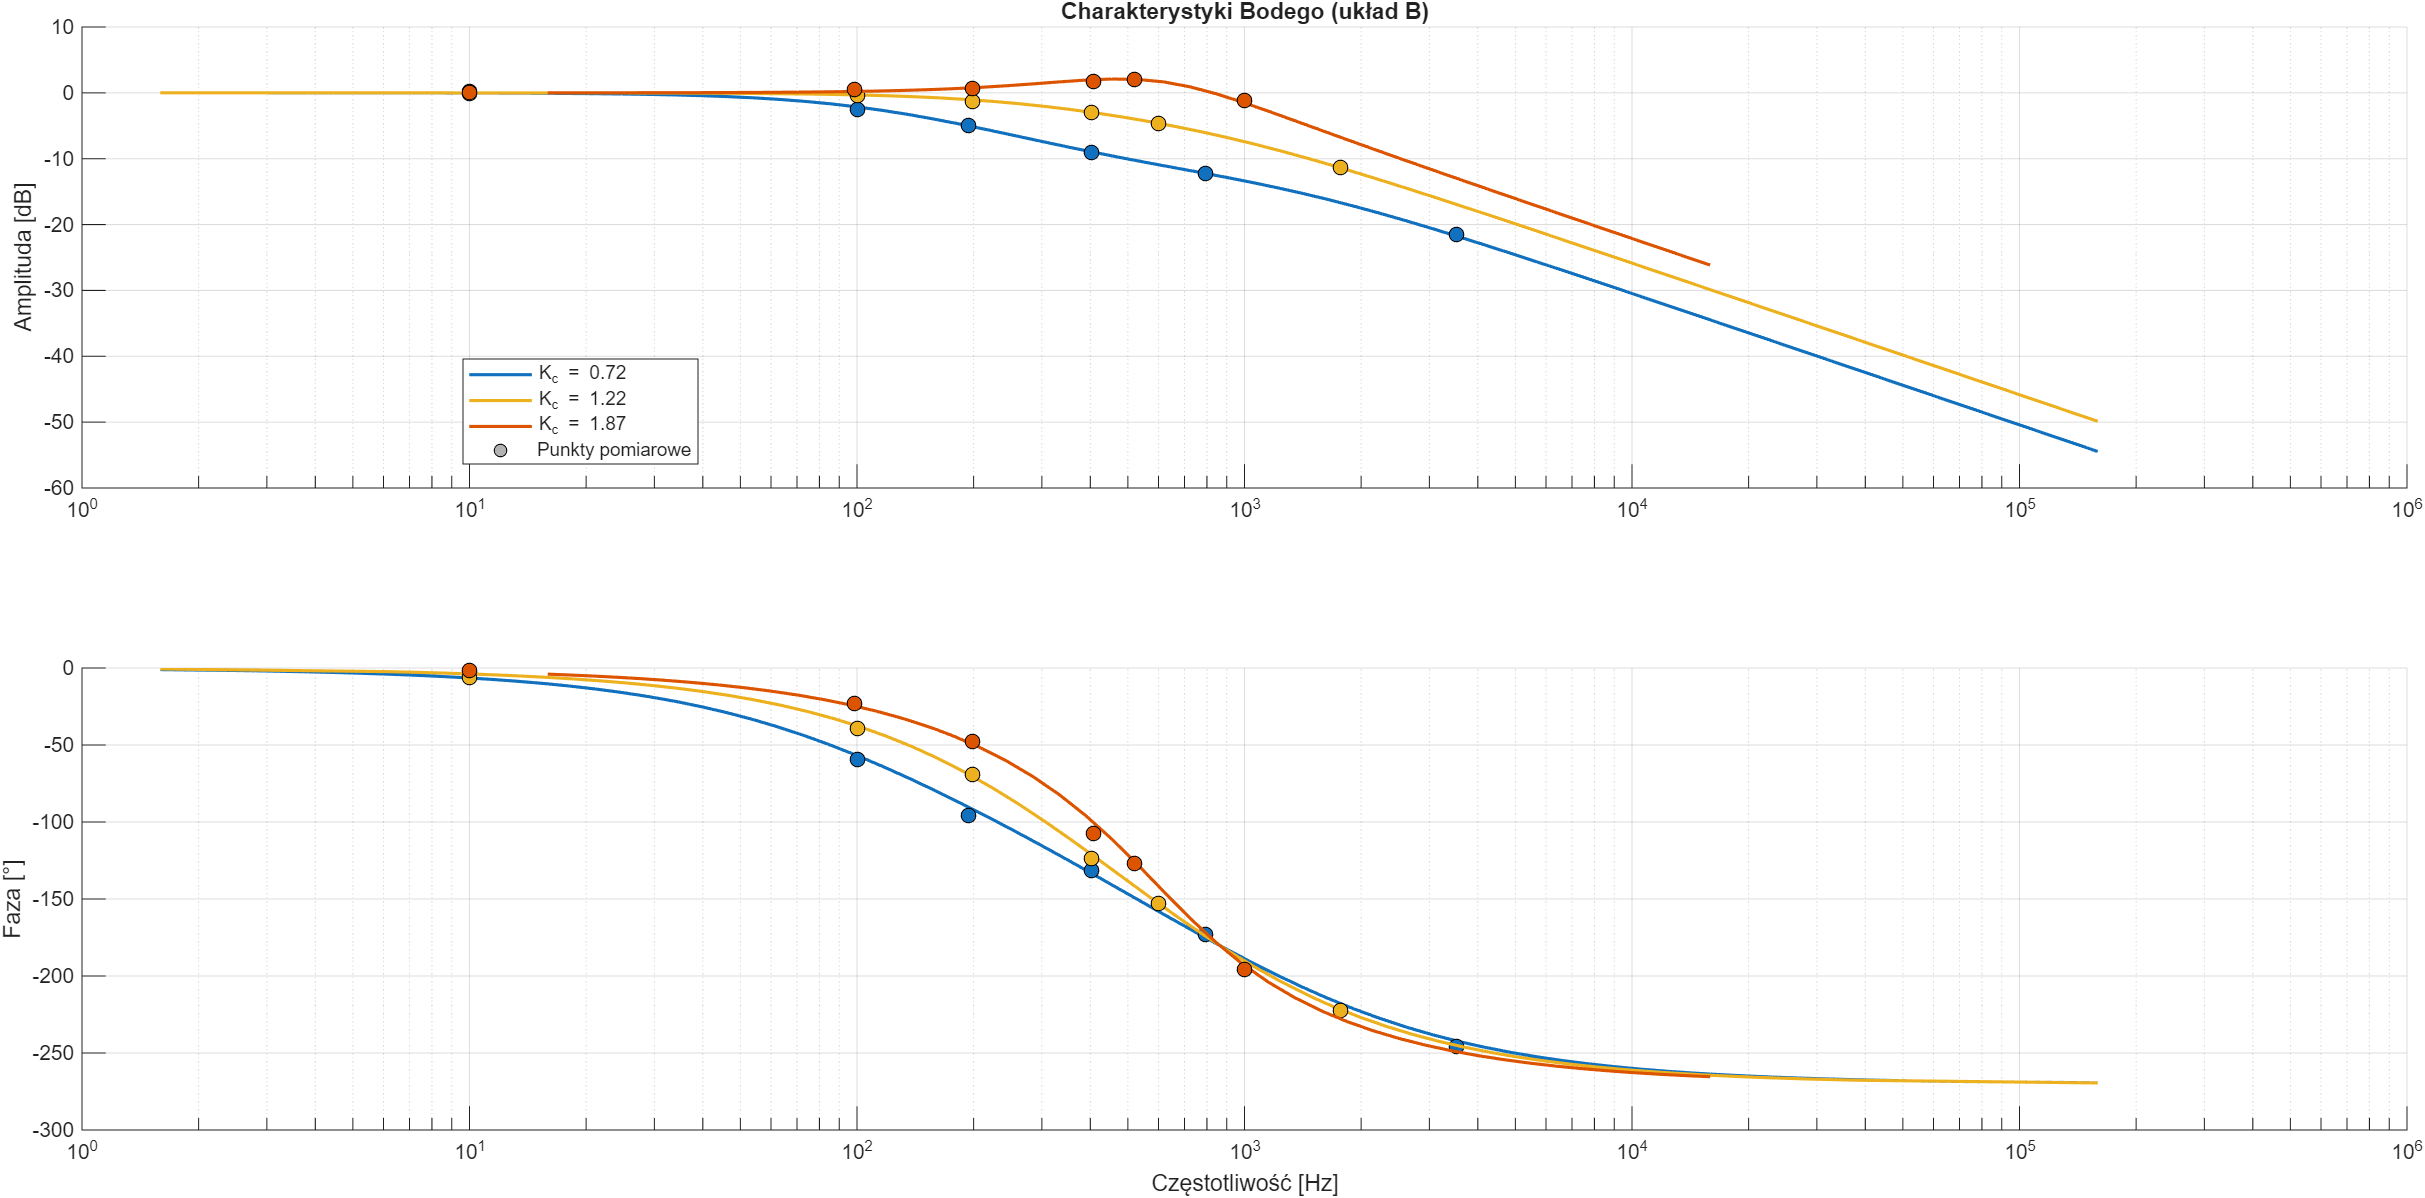
\includegraphics[width=1\linewidth]{zdjecia/Bode_ukladB.png}
		\caption{Charakterystyki Bodego układu zamkniętego (B).}
		\label{fig:Bode_ukladB}
	\end{figure}
	
	Charakterystyki Bodego układu zamkniętego (Rys. 11) potwierdzają analizę. Wzrost $k_c$ podnosi pik rezonansowy. Jednak kluczowa jest charakterystyka fazowa – człon nieminimalnofazowy wprowadza dodatkowe, nieliniowe opóźnienie fazowe. Faza spada znacznie poniżej -180°, co drastycznie redukuje zapas fazy i jest główną przyczyną niestabilności układu.
	
	\subsection{Charakterystyki Nyquista}
	
	\begin{figure}[H]
		\centering
		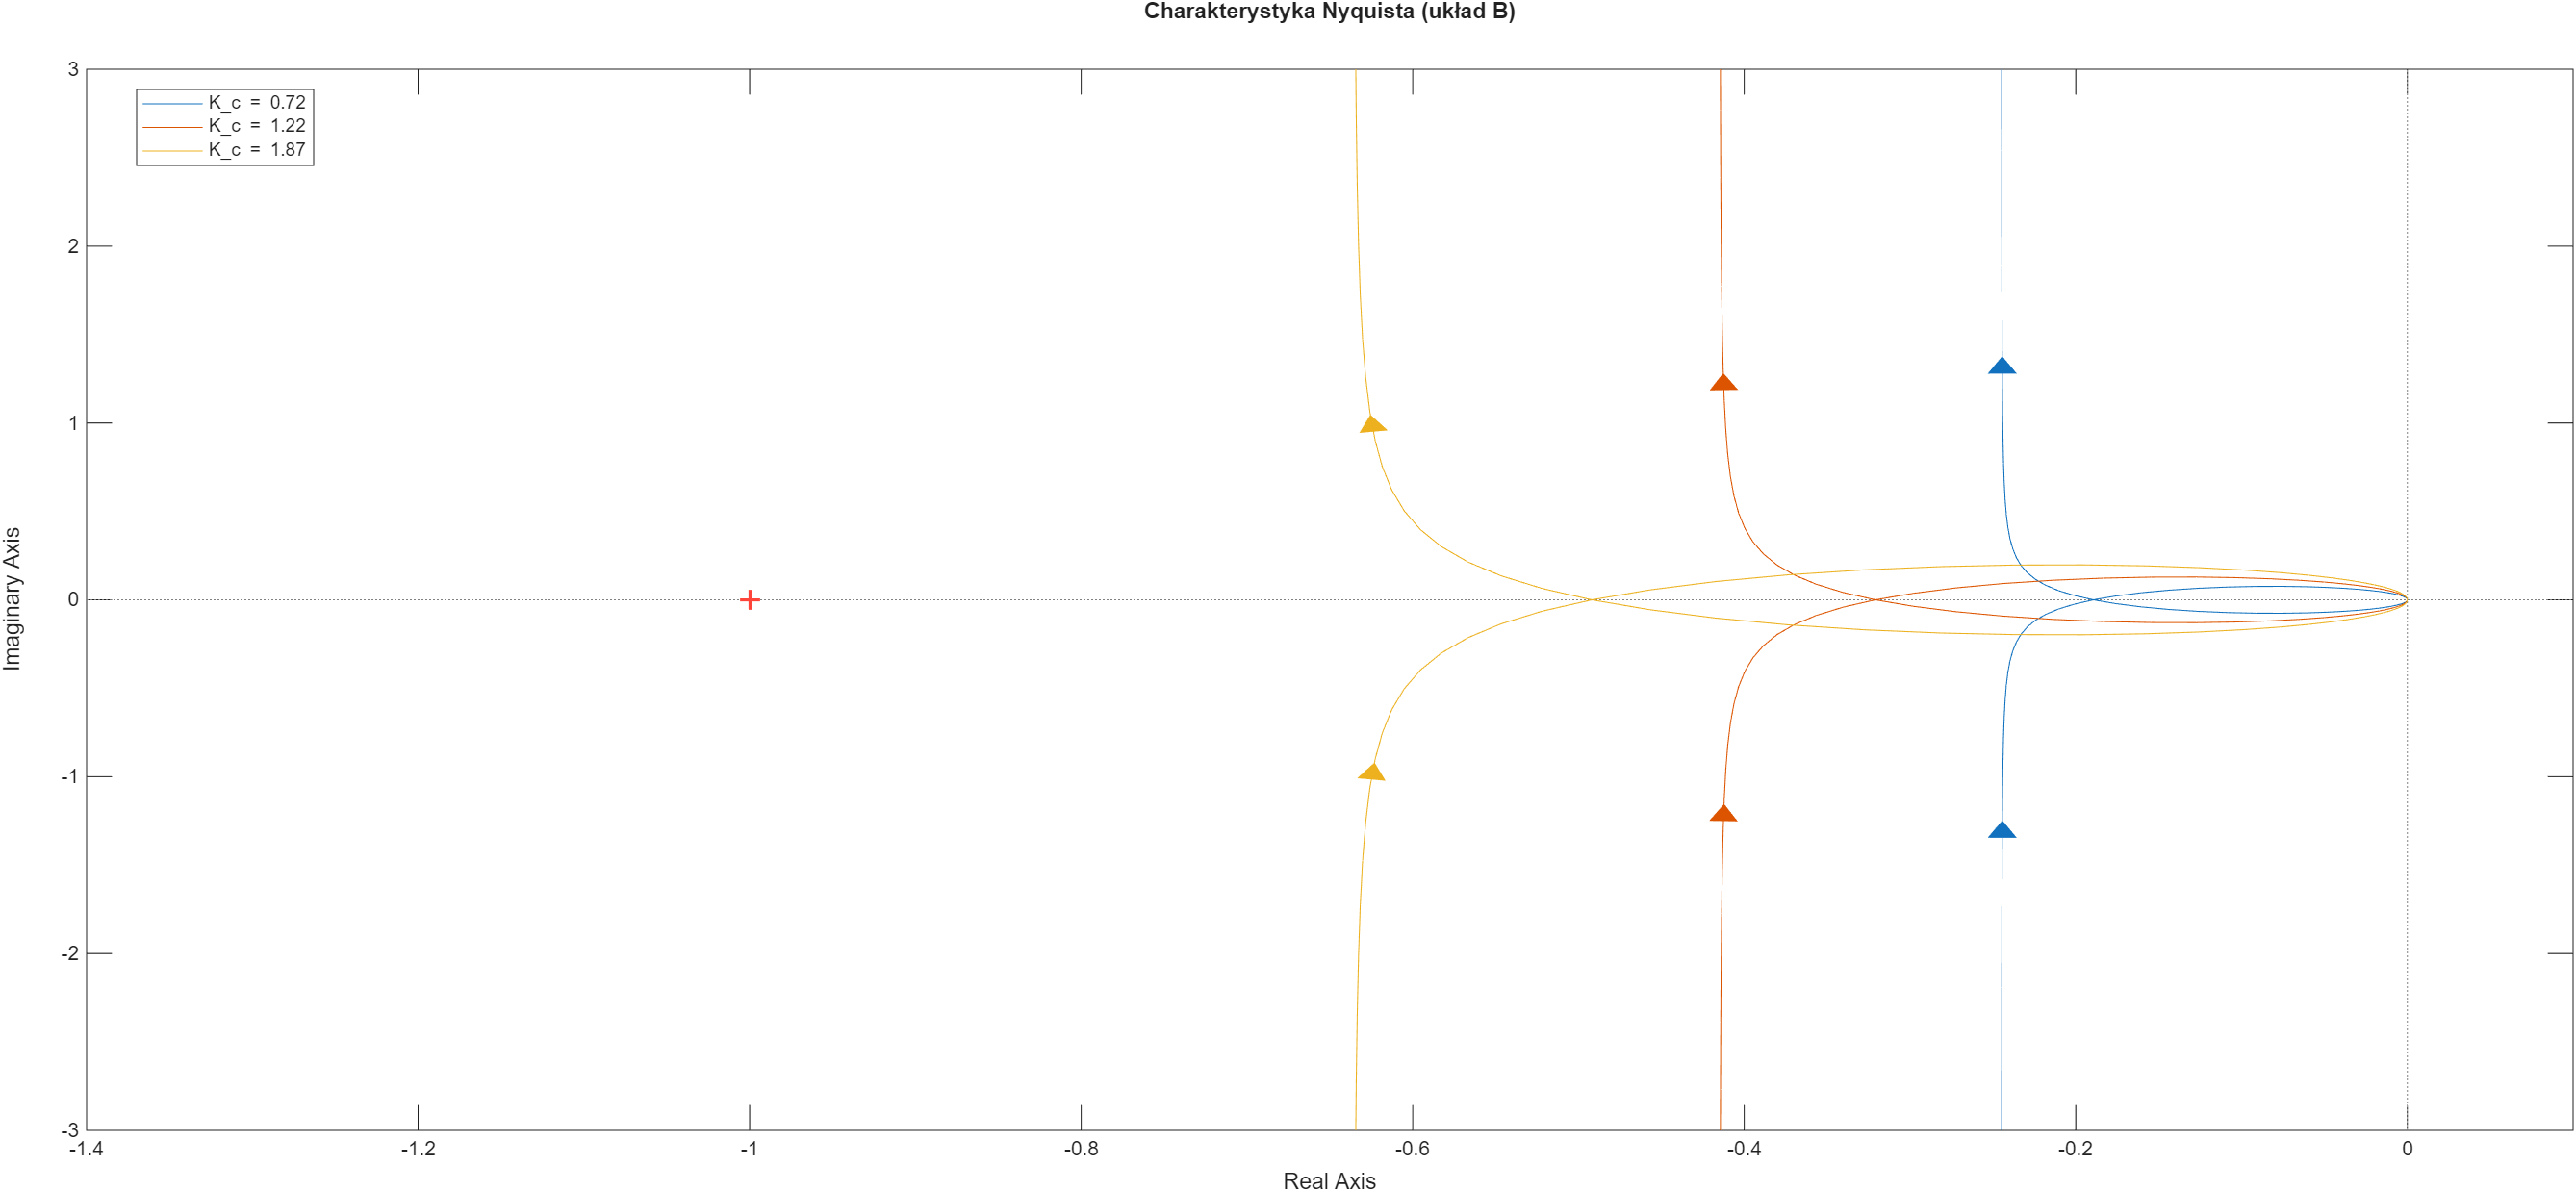
\includegraphics[width=0.8\linewidth]{zdjecia/NQ_ukladB.png}
		\caption{Charakterystyka Nyquista układu otwartego (B).}
		\label{fig:NQ_ukladB}
	\end{figure}
	
	Wykresy Nyquista układu otwartego (Rys. 12) ilustrują problem stabilności układu. Z powodu dodatkowego opóźnienia fazowego, wykres zawija się i dla rosnącego $k_c$ bardzo szybko zbliża się do punktu krytycznego (-1, 0j). Potwierdza to wnioski z linii pierwiastkowych: układ ma bardzo mały margines wzmocnienia i staje się niestabilny już przy niewielkich wartościach $k_c$.
	
	\subsection{Analityczne uzasadnienie wyników dla układu B (Obiekt całkujący z członem nieminimalnofazowym)}
	
	\textbf{Model obiektu:} $G_p(s) = \frac{1}{sT_i} \cdot \frac{1 - sT_x}{1 + sT_y}$. \\
	\textbf{Transmitancja układu otwartego:} $G_o(s) = k_c \cdot G_p(s) = \frac{k_c (1 - sT_x)}{sT_i (1 + sT_y)}$.
	
	\subsubsection{Dokładność sterowania (Uchyb ustalony)}
	\begin{itemize}
		\item \textbf{Uzasadnienie analityczne:} Podobnie jak w Układzie A, obecność członu całkującego $1/sT_i$ w pętli otwartej sprawia, że jest to \textbf{układ typu 1}. Z tego samego powodu (twierdzenie o wartości końcowej), \textbf{uchyb ustalony dla pobudzenia skokowego jest równy zero}.
		\[
		e_{ss} = \lim_{s \to 0} \frac{1}{1 + G_o(s)} = \lim_{s \to 0} \frac{1}{1 + \frac{k_c(1 - 0)}{sT_i(1 + 0)}} = \frac{1}{1 + \infty} = 0
		\]
		\item \textbf{Zgodność z pomiarami:} Pomiary (Rysunek \ref{fig:OdpSkokB}) potwierdziły, że \textbf{uchyb ustalony wynosił zero} dla każdej wartości $k_c$.
	\end{itemize}
	
	\subsubsection{Jakość odpowiedzi skokowej i stabilność}
	\begin{itemize}
		\item \textbf{Uzasadnienie analityczne:} Układ ten jest \textbf{nieminimalnofazowy} z powodu obecności zera $z = +1/T_x$ w prawej półpłaszczyźnie zespolonej. Równanie charakterystyczne układu zamkniętego:
		\[
		1 + G_o(s) = 0 \implies sT_i(1 + sT_y) + k_c(1 - sT_x) = 0
		\]
		\[
		s^2(T_i T_y) + s(T_i - k_c T_x) + k_c = 0
		\]
		Jest to układ \textbf{drugiego rzędu}. Z kryterium Routha-Hurwitza, dla stabilności wszystkie współczynniki muszą być dodatnie. O ile $T_i T_y > 0$ i $k_c > 0$, krytycznym warunkiem jest:
		\[
		T_i - k_c T_x > 0 \implies k_c < \frac{T_i}{T_x}
		\]
		Układ jest \textbf{warunkowo stabilny}, z wzmocnieniem granicznym $k_{gr} = T_i / T_x$. Zero w prawej półpłaszczyźnie przyciąga do siebie jedną z gałęzi linii pierwiastkowych (Rysunek \ref{fig:LP_ukladB}), powodując szybką utratę stabilności. W dziedzinie czasu, zero jest analityczną przyczyną obserwowanego \textbf{początkowego zanurkowania} (odpowiedź w kierunku przeciwnym do zadanego).
		
		\item \textbf{Zgodność z pomiarami:} Model analityczny idealnie wyjaśnia zachowanie układu. Pomiary na Rysunku \ref{fig:OdpSkokB} wykazały charakterystyczne zanurkowanie sygnału wyjściowego. Zwiększanie $k_c$ nie tylko pogłębiało to zanurkowanie, ale też gwałtownie zwiększało oscylacje (dla $k_{c3}=1.87$ układ był na granicy stabilności), co jest zgodne z istnieniem niskiego wzmocnienia granicznego $k_{gr}$.
	\end{itemize}
	
	\subsection{Wpływ wzmocnienia sterownika typu P na postać wszystkich procesów przejściowych w układzie B}
	\begin{itemize}
		\item Sygnał wyjściowy $c(t)$: Najbardziej charakterystyczną cechą jest początkowe zanurkowanie sygnału $c(t)$ w kierunku przeciwnym do wartości zadanej. Zwiększanie wzmocnienia $k_c$ ma dwojaki negatywny skutek: drastycznie pogłębia to początkowe zanurkowanie oraz znacząco zwiększa przeregulowanie i oscylacyjność. Jak pokazała analiza linii pierwiastkowych i Nyquista, układ ten bardzo szybko traci stabilność wraz ze wzrostem $k_c$.
		\item Uchyb $e(t)$: Z powodu zanurkowania $c(t)$, uchyb $e(t)$ początkowo rośnie (błąd się powiększa), zanim zacznie maleć. Wzrost $k_c$ pogłębia ten niekorzystny efekt. Proces przejściowy $e(t)$ jest silnie oscylacyjny. Podobnie jak w Układzie A, człon całkujący zapewnia jednak zerowy uchyb ustalony.
		\item Sygnał sterujący $u(t)$: Wzrost $k_c$ prowadzi do bardzo agresywnego sygnału $u(t)$. Sterownik, reagując na rosnący błąd (spowodowany zanurkowaniem), generuje bardzo duży sygnał sterujący, który następnie prowadzi do gwałtownego przeregulowania.
	\end{itemize}
	
	\bigskip \hrule \bigskip
	
	\section{Układ D}
	
	Ostatni badany układ to układ regulacji z zakłóceniem, składający się ze sterownika proporcjonalnego (P) i obiektu inercyjnego pierwszego rzędu.
	
	Na podstawie identyfikacji przeprowadzonej w ćwiczeniu 1, przyjęto następujące parametry modeli:
	\begin{itemize}
		\item Człon inercyjny 1 rzędu: $G(s) = \frac{k_p}{1+sT_p}$, gdzie $k_p = 0,871$ i $T_p = 0,78 \text{ ms}$.
	\end{itemize}
	
	Badania przeprowadzono dla trzech wartości wzmocnienia \(k_c\), obliczonych ze wzoru \(k_c = 0,47 + n/2\):
	\begin{itemize}
		\item Dla \(n_1 = 1,1\): $k_{c1} = 0,47 + 1,1 / 2 = 0,47 + 0,55 = \textbf{1,02}$
		\item Dla \(n_2 = 4,0\): $k_{c2} = 0,47 + 4,0 / 2 = 0,47 + 2,00 = \textbf{2,47}$
		\item Dla \(n_3 = 8,0\): $k_{c3} = 0,47 + 8,0 / 2 = 0,47 + 4,00 = \textbf{4,47}$
	\end{itemize}
	
	\subsection{Odpowiedzi skokowe}
	Na poniższym wykresie przedstawiono zarejestrowane odpowiedzi skokowe układu (D) dla trzech wyznaczonych wzmocnień \(k_c\).
	
	\begin{figure}[H]
	\centering
	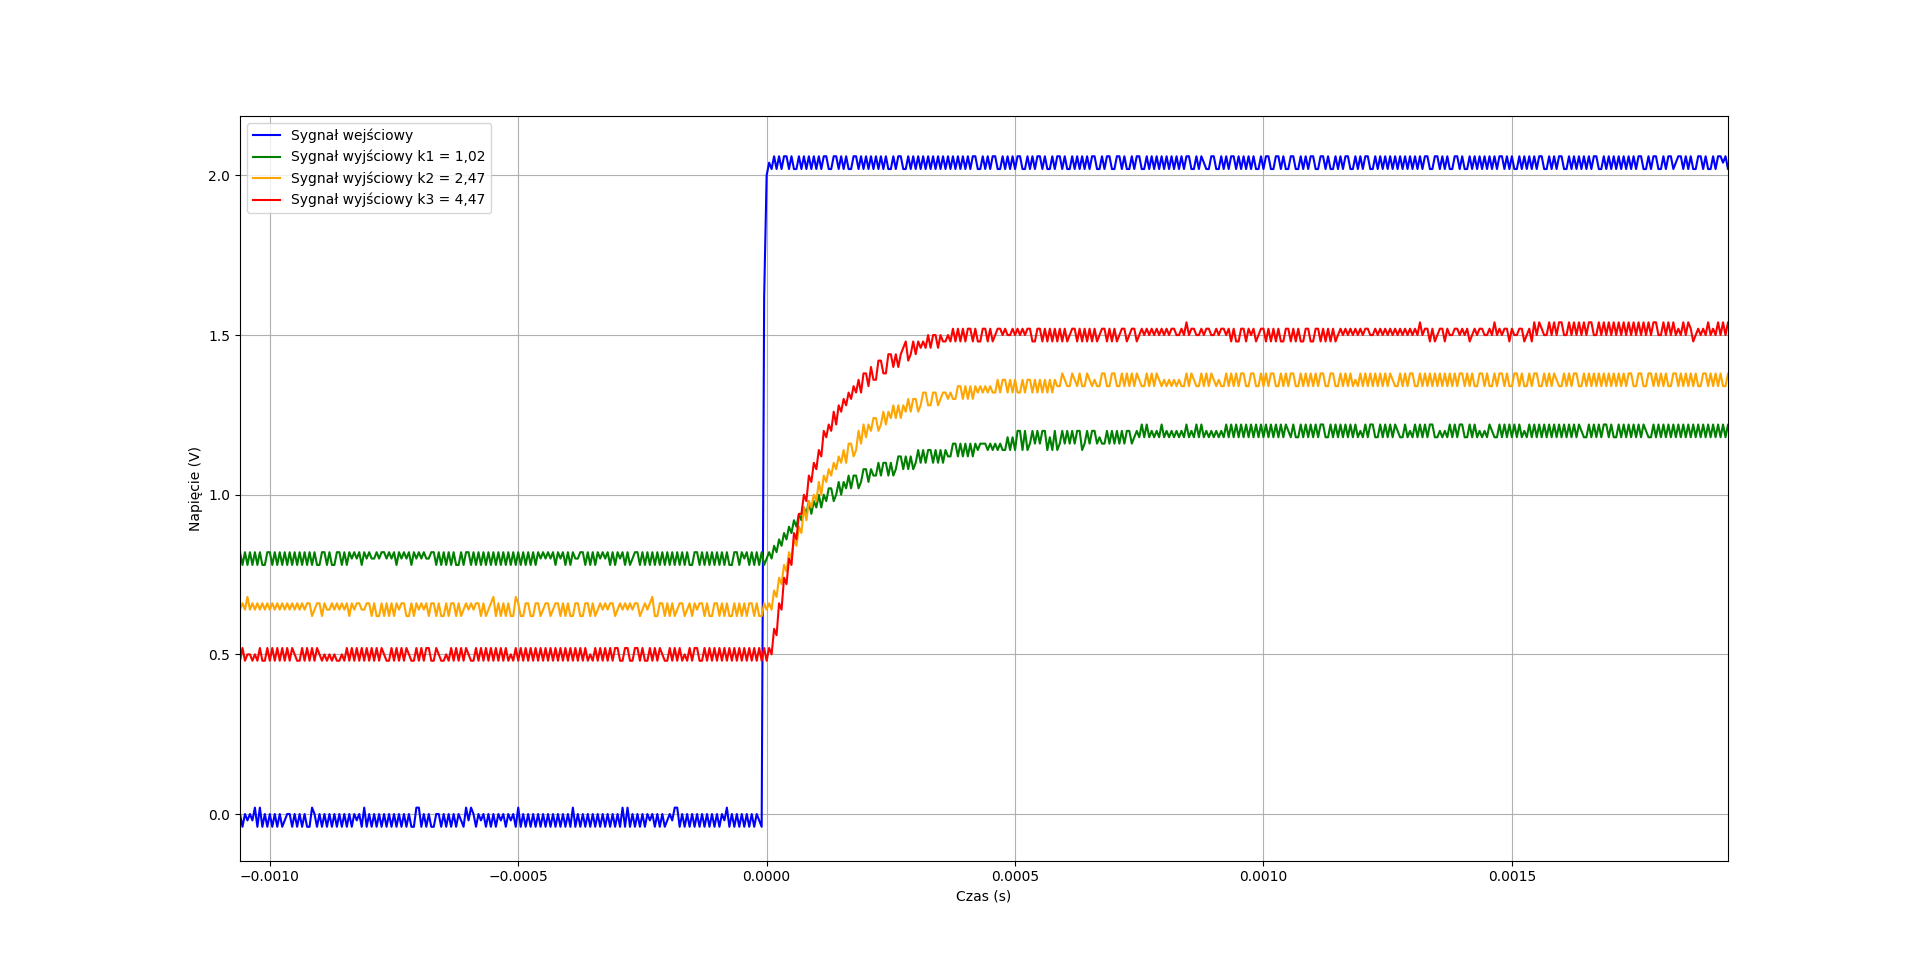
\includegraphics[width=1\linewidth]{zdjecia/OdpSkokD.png}
	\caption{Odpowiedź skokowa układu (D) przy różnych wartościach wzmocnienia \(k_c\).}
	\label{fig:OdpSkokD}
	\end{figure}
	
	Odpowiedzi skokowe dla Układu D (Rys. 13) są typowe dla układu inercyjnego pierwszego rzędu w pętli sprzężenia zwrotnego. Układ jest stabilny i nie wykazuje żadnych oscylacji ani przeregulowań, niezależnie od wartości $k_c$. Zwiększanie wzmocnienia $k_c$ przynosi dwa efekty: po pierwsze, skraca czas odpowiedzi (system staje się szybszy), a po drugie, zmniejsza uchyb ustalony. Ze względu na brak członu całkującego w pętli, uchyb ten nigdy nie jest zredukowany do zera, ale staje się mniejszy dla wyższych $k_c$.
	
	\subsection{Wpływ zakłóceń na wartość sygnału wyjściowego}
	
		Tu trzeba zasymulowac
		
	
	\subsection{Linie pierwiastkowe}
	
	\begin{figure}[H]
		\centering
		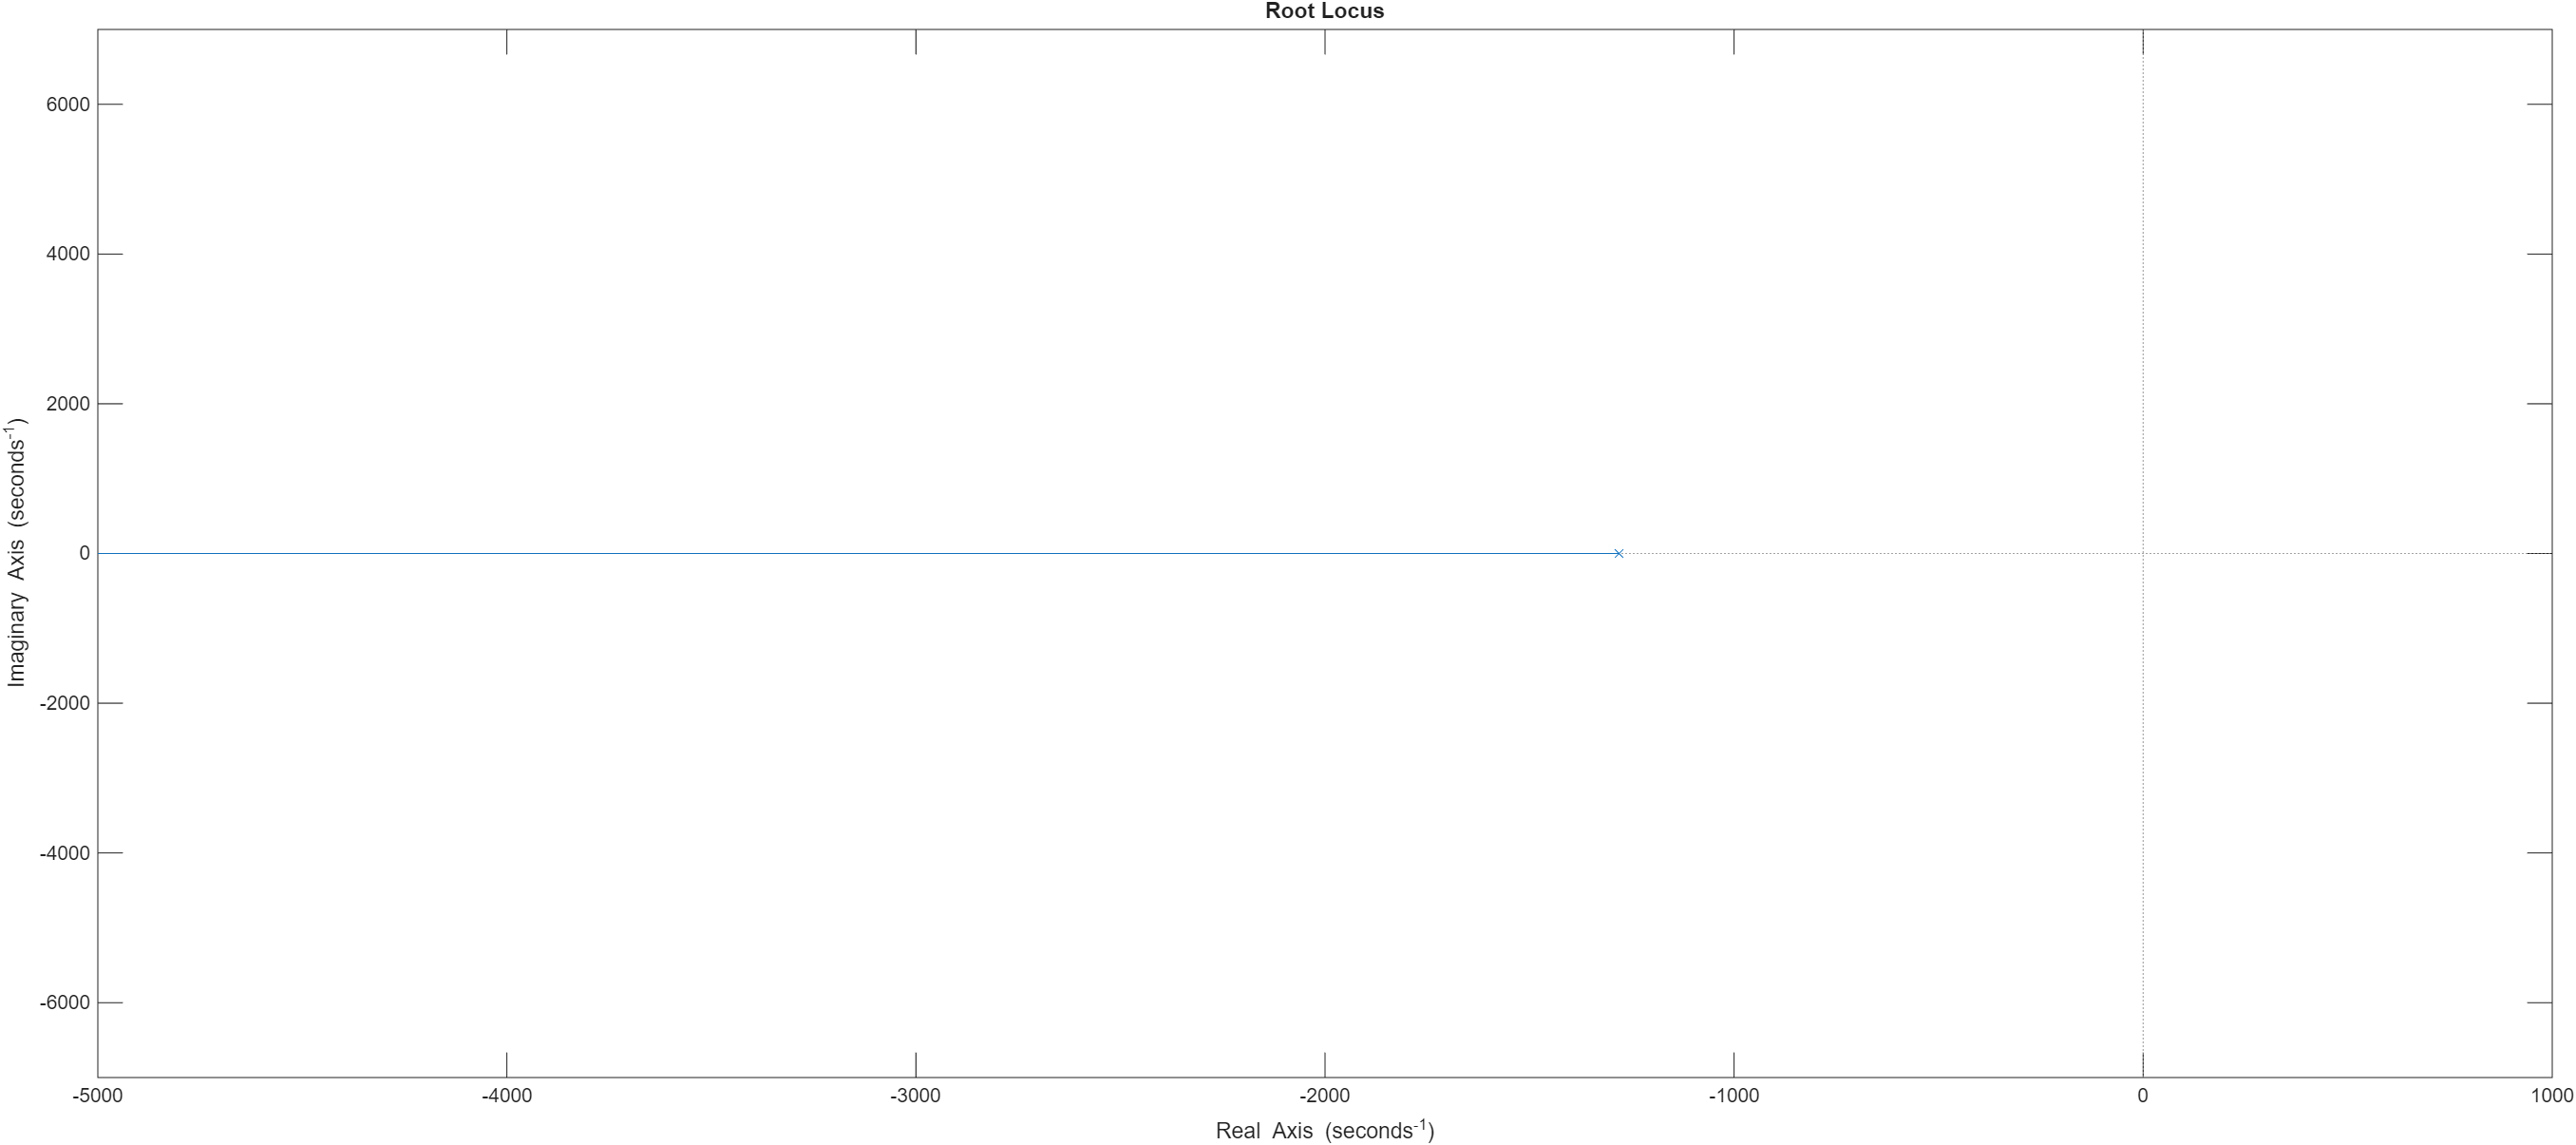
\includegraphics[width=0.8\linewidth]{zdjecia/LP_ukladD.png}
		\caption{Linie pierwiastkowe układu otwartego (D).}
		\label{fig:LP_ukladD}
	\end{figure}
	
	Linie pierwiastkowe dla Układu D (Rys. 14) są najprostsze z analizowanych. Układ otwarty ma tylko jeden biegun na ujemnej osi rzeczywistej (w punkcie $-1/T_p$). W rezultacie, linia pierwiastkowa to pojedyncza gałąź biegnąca od tego bieguna w lewo, w kierunku $-\infty$. Ponieważ biegun układu zamkniętego zawsze pozostaje na ujemnej osi rzeczywistej i nigdy nie zbliża się do osi urojonej, system jest bezwarunkowo stabilny i nieoscylacyjny dla każdej dodatniej wartości $k_c$.
	
	\subsection{Charakterystyki Bodego}
	
	\begin{figure}[H]
		\centering
		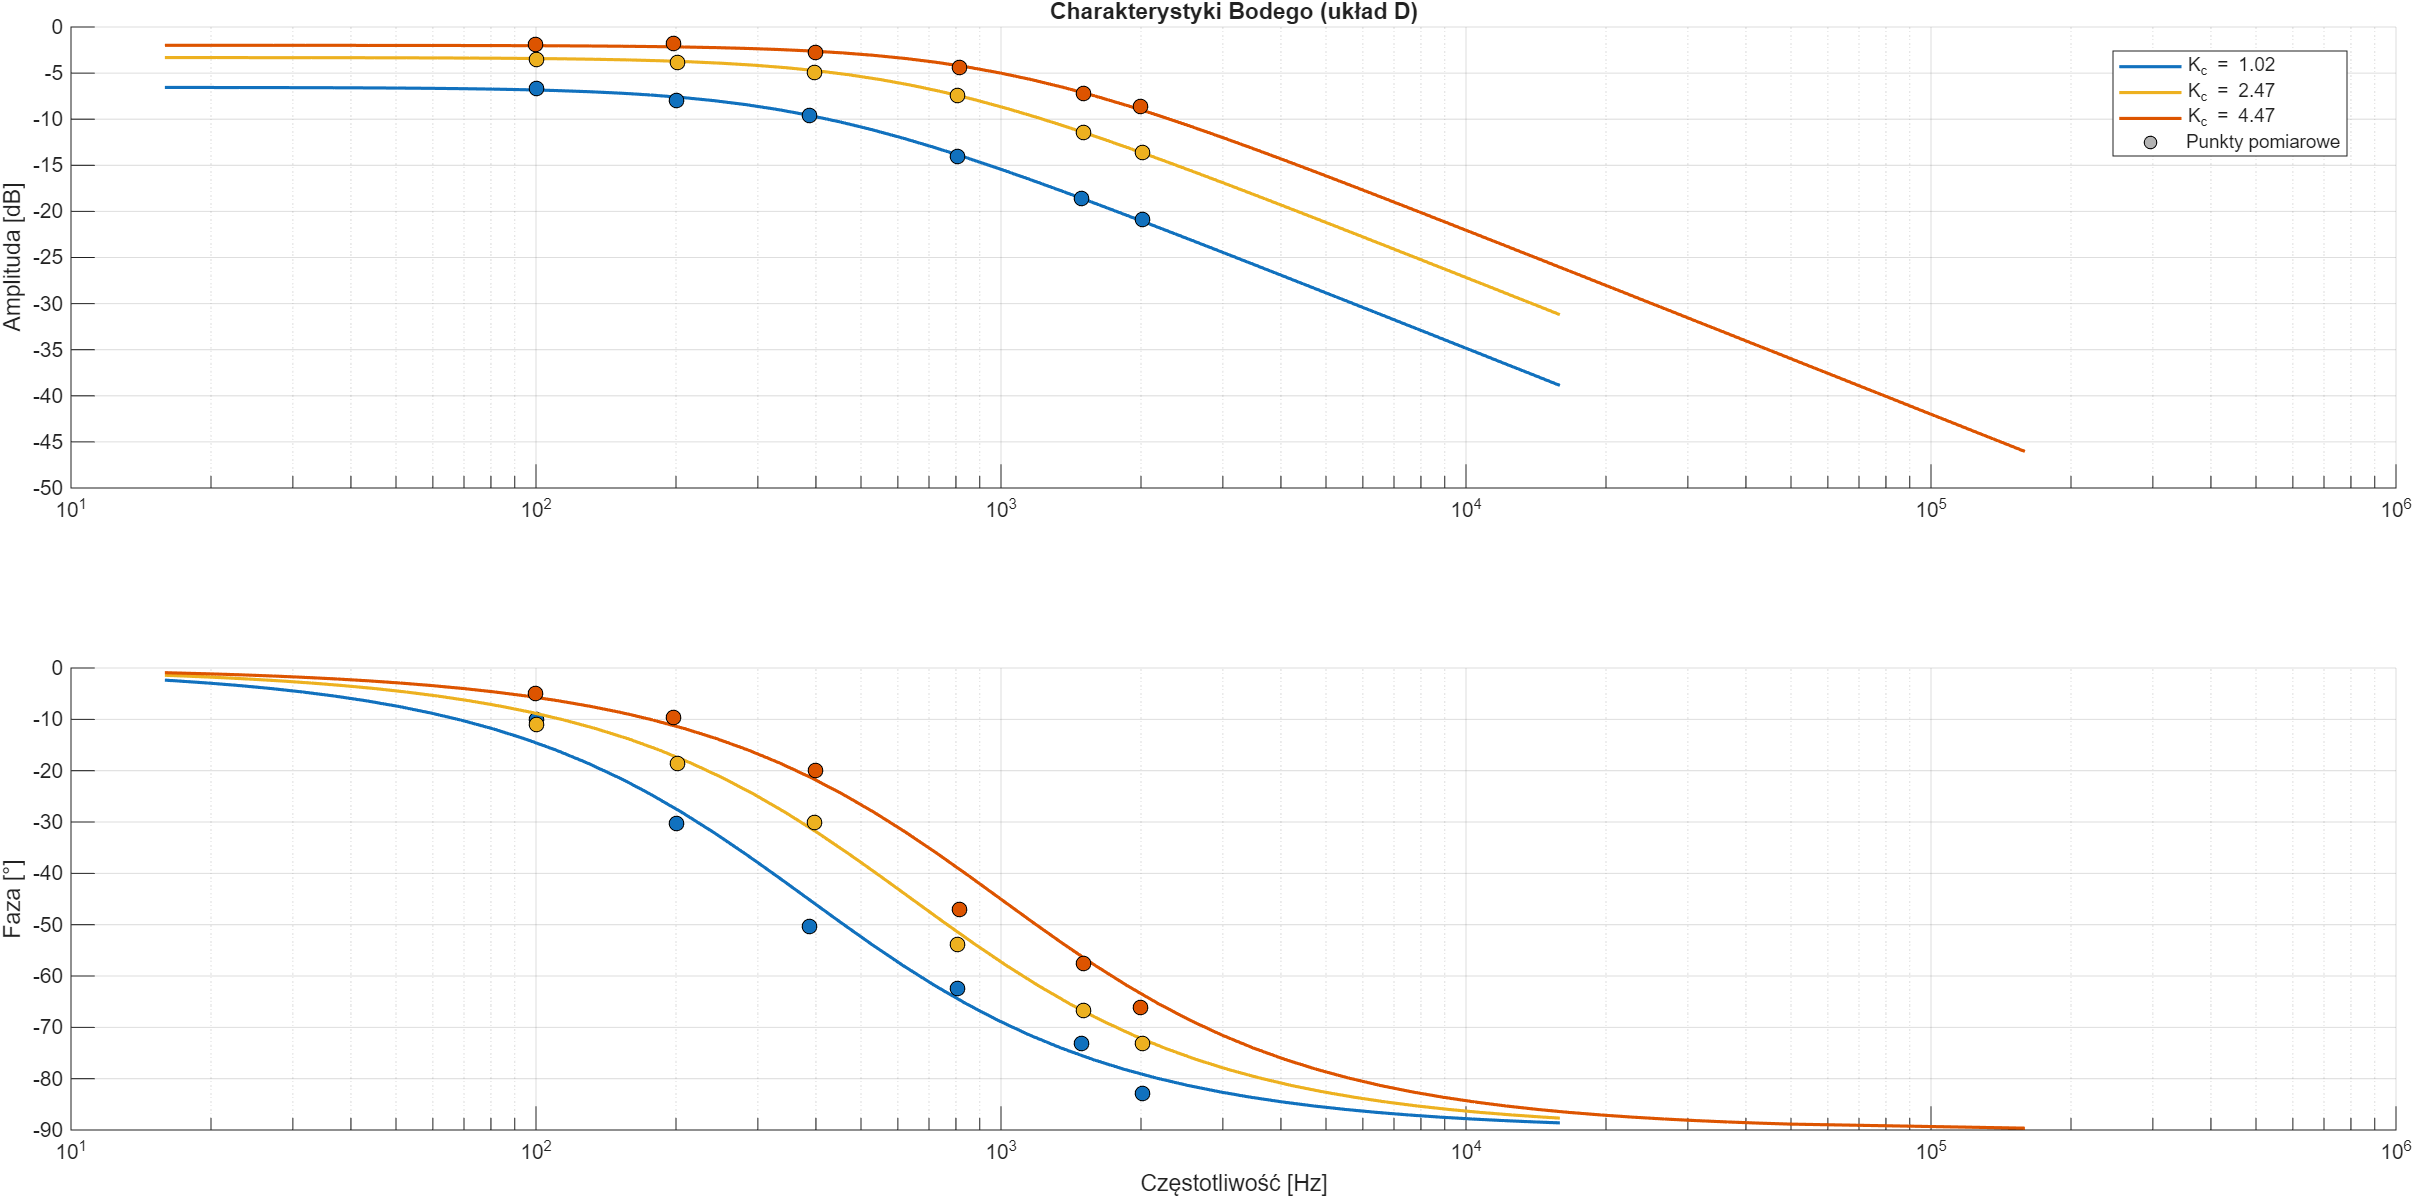
\includegraphics[width=1\linewidth]{zdjecia/Bode_ukladD.png}
		\caption{Charakterystyki Bodego układu zamkniętego (D).}
		\label{fig:Bode_ukladD}
	\end{figure}
	
	Charakterystyki Bodego układu zamkniętego (Rys. 15) pokazują, że układ działa jak filtr dolnoprzepustowy. Zwiększanie $k_c$ przesuwa całą charakterystykę amplitudową w górę i poszerza pasmo przenoszenia. Szersze pasmo oznacza, że układ szybciej reaguje na zmiany, co jest w pełni zgodne z szybszym czasem narastania widocznym na odpowiedziach skokowych (Rys. 13). Charakterystyka fazowa pokazuje maksymalne przesunięcie -90°, co potwierdza brak oscylacji.
	
	\subsection{Charakterystyki Nyquista}
	
	\begin{figure}[H]
		\centering
		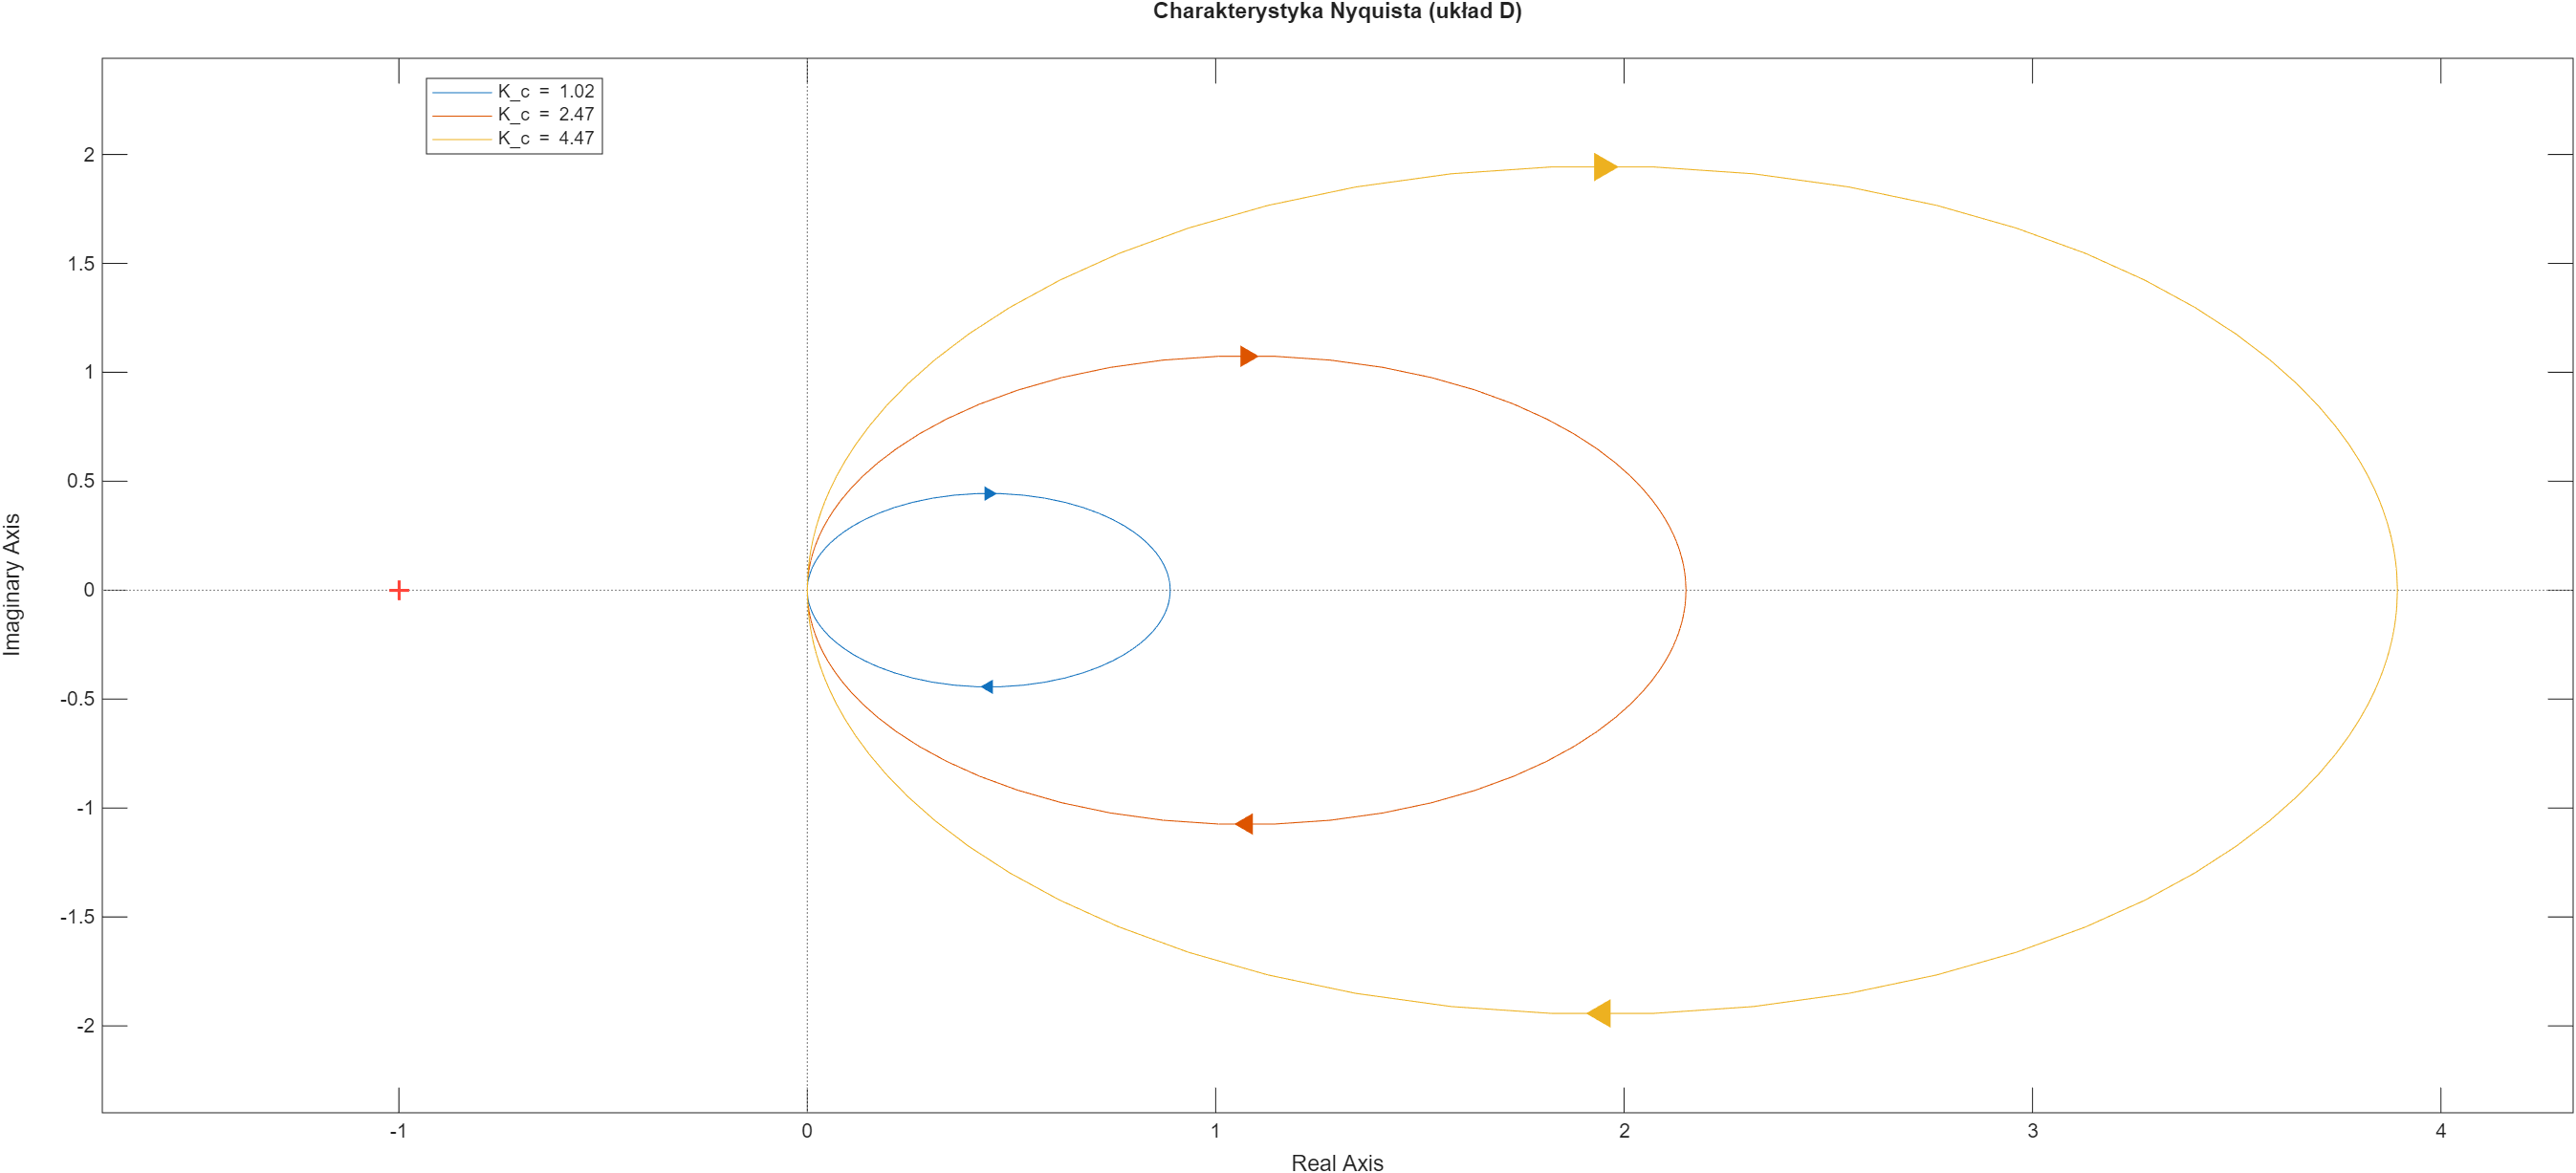
\includegraphics[width=0.8\linewidth]{zdjecia/NQ_ukladD.png}
		\caption{Charakterystyka Nyquista układu otwartego (D).}
		\label{fig:NQ_ukladD}
	\end{figure}
	
	Wykres Nyquista dla układu otwartego (Rys. 16) to prosty półokrąg leżący w całości w prawej półpłaszczyźnie (przesunięty o wartość wzmocnienia $k_c \cdot k_p$). Wzrost $k_c$ jedynie powiększa ten półokrąg. Wykres ten nigdy, nawet dla nieskończonego wzmocnienia, nie zbliży się do punktu krytycznego (-1, 0j). Oznacza to, że układ posiada nieskończony zapas wzmocnienia i fazy, co czyni go bezwarunkowo stabilnym, co potwierdzają wszystkie pozostałe analizy.
	
	\subsection{Analityczne uzasadnienie wyników dla układu D (Obiekt inercyjny I rzędu)}
	
	\textbf{Model obiektu:} $G_p(s) = \frac{k_p}{1 + sT_p}$. \\
	\textbf{Transmitancja układu otwartego:} $G_o(s) = k_c \cdot G_p(s) = \frac{k_c k_p}{1 + sT_p}$.
	
	\subsubsection{Dokładność sterowania (Uchyb ustalony)}
	\begin{itemize}
		\item \textbf{Uzasadnienie analityczne:} Układ otwarty $G_o(s)$ nie posiada bieguna w początku układu (brak członu całkującego). Jest to \textbf{układ typu 0}. Uchyb ustalony dla pobudzenia skokowego wynosi:
		\[
		e_{ss} = \lim_{s \to 0} \frac{1}{1 + G_o(s)} = \frac{1}{1 + \lim_{s \to 0} \frac{k_c k_p}{1 + sT_p}} = \frac{1}{1 + k_c k_p}
		\]
		Uchyb jest \textbf{niezerowy}, a jego wartość jest odwrotnie proporcjonalna do wzmocnienia pętli $k_c k_p$. Zwiększanie $k_c$ powoduje \textbf{zmniejszenie uchybu ustalonego}.
		
		\item \textbf{Zgodność z pomiarami:} Pomiary (Rysunek \ref{fig:OdpSkokD}) w pełni to potwierdzają. Zaobserwowano, że uchyb ustalony \textbf{nigdy nie osiąga zera}, ale jego wartość \textbf{maleje wraz ze wzrostem $k_c$}.
	\end{itemize}
	
	\subsubsection{Jakość odpowiedzi skokowej i stabilność}
	\begin{itemize}
		\item \textbf{Uzasadnienie analityczne:} Transmitancja układu zamkniętego $G_z(s) = \frac{G_o(s)}{1 + G_o(s)}$ ma postać:
		\[
		G_z(s) = \frac{\frac{k_c k_p}{1 + sT_p}}{1 + \frac{k_c k_p}{1 + sT_p}} = \frac{k_c k_p}{1 + sT_p + k_c k_p} = \frac{\frac{k_c k_p}{1 + k_c k_p}}{1 + s \frac{T_p}{1 + k_c k_p}}
		\]
		Jest to \textbf{obiekt inercyjny pierwszego rzędu} o wzmocnieniu $K_z = \frac{k_c k_p}{1 + k_c k_p}$ i stałej czasowej $T_z = \frac{T_p}{1 + k_c k_p}$. Układ posiada tylko jeden, rzeczywisty biegun ujemny $s = -1/T_z$. Taki układ jest \textbf{zawsze stabilny (bezwarunkowo)} i z natury \textbf{nie może wykazywać oscylacji ani przeregulowań}. Wzrost $k_c$ powoduje zmniejszenie stałej czasowej $T_z$, co oznacza \textbf{przyspieszenie odpowiedzi} systemu.
		
		\item \textbf{Zgodność z pomiarami:} Wyniki pomiarów (Rysunek \ref{fig:OdpSkokD}) są w idealnej zgodzie z modelem. Stwierdzono, że układ \textbf{nie wykazuje żadnych oscylacji ani przeregulowań niezależnie od $k_c$}. Zaobserwowano również, że \textbf{zwiększanie $k_c$ skraca czas odpowiedzi}. Analiza linii pierwiastkowych (Rys. \ref{fig:LP_ukladD}) i Nyquista (Rys. \ref{fig:NQ_ukladD}) również potwierdza bezwarunkową stabilność.
	\end{itemize}
	
	\subsection{Wpływ wzmocnienia sterownika typu P na postać wszystkich procesów przejściowych w układzie D}
	\begin{itemize}
		\item Sygnał wyjściowy $c(t)$: Zwiększanie $k_c$ przynosi wyłącznie pozytywne efekty dla procesu przejściowego: skraca czas odpowiedzi (system staje się szybszy). Co kluczowe, w tym układzie wzrost $k_c$ nie powoduje żadnych przeregulowań ani oscylacji. Analiza linii pierwiastkowych potwierdziła, że biegun układu zamkniętego zawsze pozostaje na ujemnej osi rzeczywistej, co gwarantuje bezwarunkową stabilność i aperiodyczność odpowiedzi.
		\item Uchyb $e(t)$: Proces przejściowy $e(t)$ również staje się szybszy – uchyb szybciej stabilizuje się na swojej wartości ustalonej. W przeciwieństwie do układów A i B, układ ten posiada niezerowy uchyb ustalony. Zwiększanie $k_c$ ma jednak korzystny wpływ na dokładność, zmniejszając wartość tego uchybu.
		\item Sygnał sterujący $u(t)$: Wzrost $k_c$ skutkuje silniejszą reakcją początkową (większe $u(0)$), co przekłada się na szybsze narastanie $c(t)$. Proces przejściowy $u(t)$ jest, podobnie jak $e(t)$, aperiodyczny i stabilizuje się na niezerowej wartości.
		\item Sygnał $a(t)$: W schemacie układu sygnał $a(t)$ jest sumą sygnału sterującego $u(t)$ i zakłócenia $d(t)$. W analizie odpowiedzi skokowej (gdzie $d(t)=0$), proces przejściowy $a(t)$ jest tożsamy z procesem przejściowym $u(t)$.
	\end{itemize}
	
	\subsection{Charakterystyki amplitudowe}
		
		Do przeprowadzenia symulacji dobraliśmy wzmocnienie układu o wartości $k_c = 1.22$.
				
		\begin{figure}[H]
			\centering
			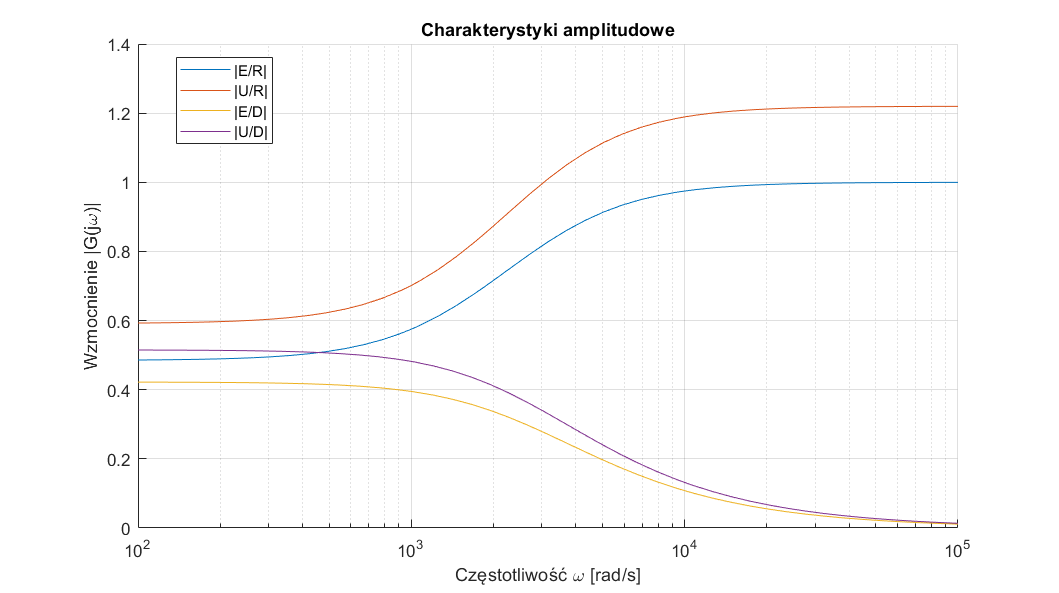
\includegraphics[width=0.8\linewidth]{zdjecia/char_czest_ukladu_D.png}
			\caption{Charakterystyka Nyquista układu otwartego (D).}
			\label{fig:char_czest_ukladu_D}
		\end{figure}
		
		Analiza przedstawionych charakterystyk amplitudowych pozwala stwierdzić, że zaprojektowany układ z regulatorem proporcjonalnym (P) wykazuje uchyb ustalony – wzmocnienie $|G_{re}(j\omega)|$ (linia niebieska) dla niskich częstotliwości stabilizuje się na poziomie ok. 0.5, a nie dąży do zera. Oznacza to, że układ nie jest w stanie idealnie śledzić wolnozmiennych sygnałów zadanych $r(t)$. Zdolność ta dodatkowo pogarsza się wraz ze wzrostem częstotliwości, a dla $\omega > 10^4$ rad/s system praktycznie przestaje nadążać za wartością zadaną ($|G_{re}(j\omega)| \approx 1$). Podobnie, system wykazuje ograniczoną zdolność do tłumienia zakłóceń $d(t)$ w paśmie niskich częstotliwości, co obrazuje charakterystyka $|G_{de}(j\omega)|$| (linia żółta, która odpowiada również $|G_{dc}(j\omega)|$), mająca wzmocnienie ok. 0.43. Wskazuje to na niezerowy wpływ stałych lub wolnozmiennych zakłóceń na sygnał wyjściowy $c(t)$. Zaletą układu jest natomiast skuteczne filtrowanie zakłóceń o wysokich częstotliwościach, gdzie wzmocnienie $|G_{de}(j\omega)|$ wyraźnie spada do zera. Charakterystyki sygnału sterującego $u(t)$ ($|G_{ru}(j\omega)|$ i $|G_{ud}(j\omega)|$) pokazują, że regulator najaktywniej działa w paśmie niskich i średnich częstotliwości, aby przeciwdziałać błędom i zakłóceniom, jednocześnie (co jest korzystne) ignorując szumy o wysokiej częstotliwości.
			
	\section{Wnioski}
	Tutaj wnioski
	
\end{document}